\documentclass[twoside]{book}

% Packages required by doxygen
\usepackage{fixltx2e}
\usepackage{calc}
\usepackage{doxygen}
\usepackage[export]{adjustbox} % also loads graphicx
\usepackage{graphicx}
\usepackage[utf8]{inputenc}
\usepackage{makeidx}
\usepackage{multicol}
\usepackage{multirow}
\PassOptionsToPackage{warn}{textcomp}
\usepackage{textcomp}
\usepackage[nointegrals]{wasysym}
\usepackage[table]{xcolor}

% Font selection
\usepackage[T1]{fontenc}
\usepackage[scaled=.90]{helvet}
\usepackage{courier}
\usepackage{amssymb}
\usepackage{sectsty}
\renewcommand{\familydefault}{\sfdefault}
\allsectionsfont{%
  \fontseries{bc}\selectfont%
  \color{darkgray}%
}
\renewcommand{\DoxyLabelFont}{%
  \fontseries{bc}\selectfont%
  \color{darkgray}%
}
\newcommand{\+}{\discretionary{\mbox{\scriptsize$\hookleftarrow$}}{}{}}

% Page & text layout
\usepackage{geometry}
\geometry{%
  a4paper,%
  top=2.5cm,%
  bottom=2.5cm,%
  left=2.5cm,%
  right=2.5cm%
}
\tolerance=750
\hfuzz=15pt
\hbadness=750
\setlength{\emergencystretch}{15pt}
\setlength{\parindent}{0cm}
\setlength{\parskip}{3ex plus 2ex minus 2ex}
\makeatletter
\renewcommand{\paragraph}{%
  \@startsection{paragraph}{4}{0ex}{-1.0ex}{1.0ex}{%
    \normalfont\normalsize\bfseries\SS@parafont%
  }%
}
\renewcommand{\subparagraph}{%
  \@startsection{subparagraph}{5}{0ex}{-1.0ex}{1.0ex}{%
    \normalfont\normalsize\bfseries\SS@subparafont%
  }%
}
\makeatother

% Headers & footers
\usepackage{fancyhdr}
\pagestyle{fancyplain}
\fancyhead[LE]{\fancyplain{}{\bfseries\thepage}}
\fancyhead[CE]{\fancyplain{}{}}
\fancyhead[RE]{\fancyplain{}{\bfseries\leftmark}}
\fancyhead[LO]{\fancyplain{}{\bfseries\rightmark}}
\fancyhead[CO]{\fancyplain{}{}}
\fancyhead[RO]{\fancyplain{}{\bfseries\thepage}}
\fancyfoot[LE]{\fancyplain{}{}}
\fancyfoot[CE]{\fancyplain{}{}}
\fancyfoot[RE]{\fancyplain{}{\bfseries\scriptsize Generated by Doxygen }}
\fancyfoot[LO]{\fancyplain{}{\bfseries\scriptsize Generated by Doxygen }}
\fancyfoot[CO]{\fancyplain{}{}}
\fancyfoot[RO]{\fancyplain{}{}}
\renewcommand{\footrulewidth}{0.4pt}
\renewcommand{\chaptermark}[1]{%
  \markboth{#1}{}%
}
\renewcommand{\sectionmark}[1]{%
  \markright{\thesection\ #1}%
}

% Indices & bibliography
\usepackage{natbib}
\usepackage[titles]{tocloft}
\setcounter{tocdepth}{3}
\setcounter{secnumdepth}{5}
\makeindex

% Hyperlinks (required, but should be loaded last)
\usepackage{ifpdf}
\ifpdf
  \usepackage[pdftex,pagebackref=true]{hyperref}
\else
  \usepackage[ps2pdf,pagebackref=true]{hyperref}
\fi
\hypersetup{%
  colorlinks=true,%
  linkcolor=blue,%
  citecolor=blue,%
  unicode%
}

% Custom commands
\newcommand{\clearemptydoublepage}{%
  \newpage{\pagestyle{empty}\cleardoublepage}%
}

\usepackage{caption}
\captionsetup{labelsep=space,justification=centering,font={bf},singlelinecheck=off,skip=4pt,position=top}

%===== C O N T E N T S =====

\begin{document}

% Titlepage & ToC
\hypersetup{pageanchor=false,
             bookmarksnumbered=true,
             pdfencoding=unicode
            }
\pagenumbering{roman}
\begin{titlepage}
\vspace*{7cm}
\begin{center}%
{\Large S\+AD Framework }\\
\vspace*{1cm}
{\large Generated by Doxygen 1.8.11}\\
\end{center}
\end{titlepage}
\clearemptydoublepage
\tableofcontents
\clearemptydoublepage
\pagenumbering{arabic}
\hypersetup{pageanchor=true}

%--- Begin generated contents ---
\chapter{Namespace Index}
\section{Packages}
Here are the packages with brief descriptions (if available)\+:\begin{DoxyCompactList}
\item\contentsline{section}{\hyperlink{namespaceSAD_1_1Config__Generator}{S\+A\+D.\+Config\+\_\+\+Generator} }{\pageref{namespaceSAD_1_1Config__Generator}}{}
\item\contentsline{section}{\hyperlink{namespaceSAD_1_1Config__PointDetector}{S\+A\+D.\+Config\+\_\+\+Point\+Detector} }{\pageref{namespaceSAD_1_1Config__PointDetector}}{}
\item\contentsline{section}{\hyperlink{namespaceSAD_1_1Config__StreamDetector}{S\+A\+D.\+Config\+\_\+\+Stream\+Detector} }{\pageref{namespaceSAD_1_1Config__StreamDetector}}{}
\item\contentsline{section}{\hyperlink{namespaceSAD_1_1Main}{S\+A\+D.\+Main} }{\pageref{namespaceSAD_1_1Main}}{}
\item\contentsline{section}{\hyperlink{namespaceSAD_1_1Main__Timestamp}{S\+A\+D.\+Main\+\_\+\+Timestamp} }{\pageref{namespaceSAD_1_1Main__Timestamp}}{}
\item\contentsline{section}{\hyperlink{namespaceSAD_1_1Point__AnomalyDetector_1_1AnomalyScorer}{S\+A\+D.\+Point\+\_\+\+Anomaly\+Detector.\+Anomaly\+Scorer} }{\pageref{namespaceSAD_1_1Point__AnomalyDetector_1_1AnomalyScorer}}{}
\item\contentsline{section}{\hyperlink{namespaceSAD_1_1Point__AnomalyDetector_1_1Fit__data}{S\+A\+D.\+Point\+\_\+\+Anomaly\+Detector.\+Fit\+\_\+data} }{\pageref{namespaceSAD_1_1Point__AnomalyDetector_1_1Fit__data}}{}
\item\contentsline{section}{\hyperlink{namespaceSAD_1_1Point__AnomalyDetector_1_1lof}{S\+A\+D.\+Point\+\_\+\+Anomaly\+Detector.\+lof} }{\pageref{namespaceSAD_1_1Point__AnomalyDetector_1_1lof}}{}
\item\contentsline{section}{\hyperlink{namespaceSAD_1_1Point__AnomalyDetector_1_1LOFAnomalyScorer}{S\+A\+D.\+Point\+\_\+\+Anomaly\+Detector.\+L\+O\+F\+Anomaly\+Scorer} }{\pageref{namespaceSAD_1_1Point__AnomalyDetector_1_1LOFAnomalyScorer}}{}
\item\contentsline{section}{\hyperlink{namespaceSAD_1_1Point__AnomalyDetector_1_1PyiscAnomalyScorer}{S\+A\+D.\+Point\+\_\+\+Anomaly\+Detector.\+Pyisc\+Anomaly\+Scorer} }{\pageref{namespaceSAD_1_1Point__AnomalyDetector_1_1PyiscAnomalyScorer}}{}
\item\contentsline{section}{\hyperlink{namespaceSAD_1_1Point__AnomalyDetector_1_1PyiscAnomalyScorer__advanced}{S\+A\+D.\+Point\+\_\+\+Anomaly\+Detector.\+Pyisc\+Anomaly\+Scorer\+\_\+advanced} }{\pageref{namespaceSAD_1_1Point__AnomalyDetector_1_1PyiscAnomalyScorer__advanced}}{}
\item\contentsline{section}{\hyperlink{namespaceSAD_1_1Stream__AnomalyDetector_1_1CUSUM}{S\+A\+D.\+Stream\+\_\+\+Anomaly\+Detector.\+C\+U\+S\+UM} }{\pageref{namespaceSAD_1_1Stream__AnomalyDetector_1_1CUSUM}}{}
\item\contentsline{section}{\hyperlink{namespaceSAD_1_1Stream__AnomalyDetector_1_1DDM}{S\+A\+D.\+Stream\+\_\+\+Anomaly\+Detector.\+D\+DM} }{\pageref{namespaceSAD_1_1Stream__AnomalyDetector_1_1DDM}}{}
\item\contentsline{section}{\hyperlink{namespaceSAD_1_1Stream__AnomalyDetector_1_1Stream__Detector}{S\+A\+D.\+Stream\+\_\+\+Anomaly\+Detector.\+Stream\+\_\+\+Detector} }{\pageref{namespaceSAD_1_1Stream__AnomalyDetector_1_1Stream__Detector}}{}
\item\contentsline{section}{\hyperlink{namespaceSAD_1_1Stream__Generator_1_1Dataset__Generator}{S\+A\+D.\+Stream\+\_\+\+Generator.\+Dataset\+\_\+\+Generator} }{\pageref{namespaceSAD_1_1Stream__Generator_1_1Dataset__Generator}}{}
\item\contentsline{section}{\hyperlink{namespaceSAD_1_1Stream__Generator_1_1Generator}{S\+A\+D.\+Stream\+\_\+\+Generator.\+Generator} }{\pageref{namespaceSAD_1_1Stream__Generator_1_1Generator}}{}
\item\contentsline{section}{\hyperlink{namespaceSAD_1_1Stream__Generator_1_1Simulation__Generator}{S\+A\+D.\+Stream\+\_\+\+Generator.\+Simulation\+\_\+\+Generator} }{\pageref{namespaceSAD_1_1Stream__Generator_1_1Simulation__Generator}}{}
\item\contentsline{section}{\hyperlink{namespaceSAD_1_1Stream__Generator_1_1Timestamp__Dataset__Generator}{S\+A\+D.\+Stream\+\_\+\+Generator.\+Timestamp\+\_\+\+Dataset\+\_\+\+Generator} }{\pageref{namespaceSAD_1_1Stream__Generator_1_1Timestamp__Dataset__Generator}}{}
\end{DoxyCompactList}

\chapter{Hierarchical Index}
\section{Class Hierarchy}
This inheritance list is sorted roughly, but not completely, alphabetically\+:\begin{DoxyCompactList}
\item \contentsline{section}{S\+A\+D.\+Point\+\_\+\+Anomaly\+Detector.\+Fit\+\_\+data.\+Fit\+\_\+data}{\pageref{classSAD_1_1Point__AnomalyDetector_1_1Fit__data_1_1Fit__data}}{}
\item \contentsline{section}{S\+A\+D.\+Point\+\_\+\+Anomaly\+Detector.\+lof.\+L\+OF}{\pageref{classSAD_1_1Point__AnomalyDetector_1_1lof_1_1LOF}}{}
\item object\begin{DoxyCompactList}
\item \contentsline{section}{S\+A\+D.\+Point\+\_\+\+Anomaly\+Detector.\+Anomaly\+Scorer.\+Anomaly\+Scorer}{\pageref{classSAD_1_1Point__AnomalyDetector_1_1AnomalyScorer_1_1AnomalyScorer}}{}
\item \contentsline{section}{S\+A\+D.\+Stream\+\_\+\+Anomaly\+Detector.\+Stream\+\_\+\+Detector.\+Stream\+\_\+\+Detector}{\pageref{classSAD_1_1Stream__AnomalyDetector_1_1Stream__Detector_1_1Stream__Detector}}{}
\item \contentsline{section}{S\+A\+D.\+Stream\+\_\+\+Generator.\+Generator.\+Generator}{\pageref{classSAD_1_1Stream__Generator_1_1Generator_1_1Generator}}{}
\end{DoxyCompactList}
\item Anomaly\+Scorer\begin{DoxyCompactList}
\item \contentsline{section}{S\+A\+D.\+Point\+\_\+\+Anomaly\+Detector.\+L\+O\+F\+Anomaly\+Scorer.\+L\+O\+F\+Anomaly\+Scorer}{\pageref{classSAD_1_1Point__AnomalyDetector_1_1LOFAnomalyScorer_1_1LOFAnomalyScorer}}{}
\item \contentsline{section}{S\+A\+D.\+Point\+\_\+\+Anomaly\+Detector.\+Pyisc\+Anomaly\+Scorer.\+Pyisc\+Anomaly\+Scorer}{\pageref{classSAD_1_1Point__AnomalyDetector_1_1PyiscAnomalyScorer_1_1PyiscAnomalyScorer}}{}
\item \contentsline{section}{S\+A\+D.\+Point\+\_\+\+Anomaly\+Detector.\+Pyisc\+Anomaly\+Scorer\+\_\+advanced.\+Pyisc\+Anomaly\+Scorer\+\_\+advanced}{\pageref{classSAD_1_1Point__AnomalyDetector_1_1PyiscAnomalyScorer__advanced_1_1PyiscAnomalyScorer__advanced}}{}
\item \contentsline{section}{S\+A\+D.\+Point\+\_\+\+Anomaly\+Detector.\+S\+V\+M\+Anomaly\+Scorer.\+S\+V\+M\+Anomaly\+Scorer}{\pageref{classSAD_1_1Point__AnomalyDetector_1_1SVMAnomalyScorer_1_1SVMAnomalyScorer}}{}
\end{DoxyCompactList}
\item Generator\begin{DoxyCompactList}
\item \contentsline{section}{S\+A\+D.\+Stream\+\_\+\+Generator.\+Dataset\+\_\+\+Generator.\+Dataset\+\_\+\+Generator}{\pageref{classSAD_1_1Stream__Generator_1_1Dataset__Generator_1_1Dataset__Generator}}{}
\item \contentsline{section}{S\+A\+D.\+Stream\+\_\+\+Generator.\+Simulation\+\_\+\+Generator.\+Simulation\+\_\+\+Generator}{\pageref{classSAD_1_1Stream__Generator_1_1Simulation__Generator_1_1Simulation__Generator}}{}
\item \contentsline{section}{S\+A\+D.\+Stream\+\_\+\+Generator.\+Timestamp\+\_\+\+Dataset\+\_\+\+Generator.\+Timestamp\+\_\+\+Dataset\+\_\+\+Generator}{\pageref{classSAD_1_1Stream__Generator_1_1Timestamp__Dataset__Generator_1_1Timestamp__Dataset__Generator}}{}
\end{DoxyCompactList}
\item Stream\+\_\+\+Detector\begin{DoxyCompactList}
\item \contentsline{section}{S\+A\+D.\+Stream\+\_\+\+Anomaly\+Detector.\+C\+U\+S\+U\+M.\+C\+U\+S\+UM}{\pageref{classSAD_1_1Stream__AnomalyDetector_1_1CUSUM_1_1CUSUM}}{}
\item \contentsline{section}{S\+A\+D.\+Stream\+\_\+\+Anomaly\+Detector.\+D\+D\+M.\+D\+DM}{\pageref{classSAD_1_1Stream__AnomalyDetector_1_1DDM_1_1DDM}}{}
\item \contentsline{section}{S\+A\+D.\+Stream\+\_\+\+Anomaly\+Detector.\+F\+C\+W\+M.\+F\+C\+WM}{\pageref{classSAD_1_1Stream__AnomalyDetector_1_1FCWM_1_1FCWM}}{}
\item \contentsline{section}{S\+A\+D.\+Stream\+\_\+\+Anomaly\+Detector.\+P\+R\+A\+A\+G.\+P\+R\+A\+AG}{\pageref{classSAD_1_1Stream__AnomalyDetector_1_1PRAAG_1_1PRAAG}}{}
\end{DoxyCompactList}
\end{DoxyCompactList}

\chapter{Class Index}
\section{Class List}
Here are the classes, structs, unions and interfaces with brief descriptions\+:\begin{DoxyCompactList}
\item\contentsline{section}{\hyperlink{classSAD_1_1Point__AnomalyDetector_1_1AnomalyScorer_1_1AnomalyScorer}{S\+A\+D.\+Point\+\_\+\+Anomaly\+Detector.\+Anomaly\+Scorer.\+Anomaly\+Scorer} }{\pageref{classSAD_1_1Point__AnomalyDetector_1_1AnomalyScorer_1_1AnomalyScorer}}{}
\item\contentsline{section}{\hyperlink{classSAD_1_1Stream__AnomalyDetector_1_1CUSUM_1_1CUSUM}{S\+A\+D.\+Stream\+\_\+\+Anomaly\+Detector.\+C\+U\+S\+U\+M.\+C\+U\+S\+UM} }{\pageref{classSAD_1_1Stream__AnomalyDetector_1_1CUSUM_1_1CUSUM}}{}
\item\contentsline{section}{\hyperlink{classSAD_1_1Stream__Generator_1_1Dataset__Generator_1_1Dataset__Generator}{S\+A\+D.\+Stream\+\_\+\+Generator.\+Dataset\+\_\+\+Generator.\+Dataset\+\_\+\+Generator} }{\pageref{classSAD_1_1Stream__Generator_1_1Dataset__Generator_1_1Dataset__Generator}}{}
\item\contentsline{section}{\hyperlink{classSAD_1_1Stream__AnomalyDetector_1_1DDM_1_1DDM}{S\+A\+D.\+Stream\+\_\+\+Anomaly\+Detector.\+D\+D\+M.\+D\+DM} }{\pageref{classSAD_1_1Stream__AnomalyDetector_1_1DDM_1_1DDM}}{}
\item\contentsline{section}{\hyperlink{classSAD_1_1Stream__AnomalyDetector_1_1FCWM_1_1FCWM}{S\+A\+D.\+Stream\+\_\+\+Anomaly\+Detector.\+F\+C\+W\+M.\+F\+C\+WM} }{\pageref{classSAD_1_1Stream__AnomalyDetector_1_1FCWM_1_1FCWM}}{}
\item\contentsline{section}{\hyperlink{classSAD_1_1Point__AnomalyDetector_1_1Fit__data_1_1Fit__data}{S\+A\+D.\+Point\+\_\+\+Anomaly\+Detector.\+Fit\+\_\+data.\+Fit\+\_\+data} }{\pageref{classSAD_1_1Point__AnomalyDetector_1_1Fit__data_1_1Fit__data}}{}
\item\contentsline{section}{\hyperlink{classSAD_1_1Stream__Generator_1_1Generator_1_1Generator}{S\+A\+D.\+Stream\+\_\+\+Generator.\+Generator.\+Generator} }{\pageref{classSAD_1_1Stream__Generator_1_1Generator_1_1Generator}}{}
\item\contentsline{section}{\hyperlink{classSAD_1_1Point__AnomalyDetector_1_1lof_1_1LOF}{S\+A\+D.\+Point\+\_\+\+Anomaly\+Detector.\+lof.\+L\+OF} }{\pageref{classSAD_1_1Point__AnomalyDetector_1_1lof_1_1LOF}}{}
\item\contentsline{section}{\hyperlink{classSAD_1_1Point__AnomalyDetector_1_1LOFAnomalyScorer_1_1LOFAnomalyScorer}{S\+A\+D.\+Point\+\_\+\+Anomaly\+Detector.\+L\+O\+F\+Anomaly\+Scorer.\+L\+O\+F\+Anomaly\+Scorer} }{\pageref{classSAD_1_1Point__AnomalyDetector_1_1LOFAnomalyScorer_1_1LOFAnomalyScorer}}{}
\item\contentsline{section}{\hyperlink{classSAD_1_1Stream__AnomalyDetector_1_1PRAAG_1_1PRAAG}{S\+A\+D.\+Stream\+\_\+\+Anomaly\+Detector.\+P\+R\+A\+A\+G.\+P\+R\+A\+AG} }{\pageref{classSAD_1_1Stream__AnomalyDetector_1_1PRAAG_1_1PRAAG}}{}
\item\contentsline{section}{\hyperlink{classSAD_1_1Point__AnomalyDetector_1_1PyiscAnomalyScorer_1_1PyiscAnomalyScorer}{S\+A\+D.\+Point\+\_\+\+Anomaly\+Detector.\+Pyisc\+Anomaly\+Scorer.\+Pyisc\+Anomaly\+Scorer} }{\pageref{classSAD_1_1Point__AnomalyDetector_1_1PyiscAnomalyScorer_1_1PyiscAnomalyScorer}}{}
\item\contentsline{section}{\hyperlink{classSAD_1_1Point__AnomalyDetector_1_1PyiscAnomalyScorer__advanced_1_1PyiscAnomalyScorer__advanced}{S\+A\+D.\+Point\+\_\+\+Anomaly\+Detector.\+Pyisc\+Anomaly\+Scorer\+\_\+advanced.\+Pyisc\+Anomaly\+Scorer\+\_\+advanced} }{\pageref{classSAD_1_1Point__AnomalyDetector_1_1PyiscAnomalyScorer__advanced_1_1PyiscAnomalyScorer__advanced}}{}
\item\contentsline{section}{\hyperlink{classSAD_1_1Stream__Generator_1_1Simulation__Generator_1_1Simulation__Generator}{S\+A\+D.\+Stream\+\_\+\+Generator.\+Simulation\+\_\+\+Generator.\+Simulation\+\_\+\+Generator} }{\pageref{classSAD_1_1Stream__Generator_1_1Simulation__Generator_1_1Simulation__Generator}}{}
\item\contentsline{section}{\hyperlink{classSAD_1_1Stream__AnomalyDetector_1_1Stream__Detector_1_1Stream__Detector}{S\+A\+D.\+Stream\+\_\+\+Anomaly\+Detector.\+Stream\+\_\+\+Detector.\+Stream\+\_\+\+Detector} }{\pageref{classSAD_1_1Stream__AnomalyDetector_1_1Stream__Detector_1_1Stream__Detector}}{}
\item\contentsline{section}{\hyperlink{classSAD_1_1Point__AnomalyDetector_1_1SVMAnomalyScorer_1_1SVMAnomalyScorer}{S\+A\+D.\+Point\+\_\+\+Anomaly\+Detector.\+S\+V\+M\+Anomaly\+Scorer.\+S\+V\+M\+Anomaly\+Scorer} }{\pageref{classSAD_1_1Point__AnomalyDetector_1_1SVMAnomalyScorer_1_1SVMAnomalyScorer}}{}
\item\contentsline{section}{\hyperlink{classSAD_1_1Stream__Generator_1_1Timestamp__Dataset__Generator_1_1Timestamp__Dataset__Generator}{S\+A\+D.\+Stream\+\_\+\+Generator.\+Timestamp\+\_\+\+Dataset\+\_\+\+Generator.\+Timestamp\+\_\+\+Dataset\+\_\+\+Generator} }{\pageref{classSAD_1_1Stream__Generator_1_1Timestamp__Dataset__Generator_1_1Timestamp__Dataset__Generator}}{}
\end{DoxyCompactList}

\chapter{Namespace Documentation}
\hypertarget{namespaceSAD_1_1Config__Generator}{}\section{S\+A\+D.\+Config\+\_\+\+Generator Namespace Reference}
\label{namespaceSAD_1_1Config__Generator}\index{S\+A\+D.\+Config\+\_\+\+Generator@{S\+A\+D.\+Config\+\_\+\+Generator}}
\subsection*{Functions}
\begin{DoxyCompactItemize}
\item 
def \hyperlink{namespaceSAD_1_1Config__Generator_ae141063b2f05ef30572b428d0ce17a54}{Generate\+\_\+from\+\_\+simulation} (Normal\+\_\+\+Error, Anomaly\+\_\+\+Error, list\+\_\+distribution, type\+\_\+error, incremental=False, Number\+\_\+\+Of\+\_\+\+Train=10000)
\item 
def \hyperlink{namespaceSAD_1_1Config__Generator_a7a4f97db8a198075e635bac49c744e3e}{Generate\+\_\+from\+\_\+dataset} (filename, delimiter, normal\+\_\+class, column=-\/1, type\+\_\+error=\char`\"{}Sudden\char`\"{}, incremental=False, percentage=0.\+7)
\item 
def \hyperlink{namespaceSAD_1_1Config__Generator_a115ab2861e50a264cb48a51cbfde5340}{Generate\+\_\+from\+\_\+timestamp} (filename, delimiter=\char`\"{},  del\+\_\+timestamp\+\_\+column=True,  timestamp\+\_\+column=0,  percentage=0.\+7,  incremental=False)
\end{DoxyCompactItemize}


\subsection{Detailed Description}
\begin{DoxyVerb}:copyright: (c) 2016 Jiakun Jin
email: jiakun@kth.se
:license: LGPL?
\end{DoxyVerb}
 

\subsection{Function Documentation}
\index{S\+A\+D\+::\+Config\+\_\+\+Generator@{S\+A\+D\+::\+Config\+\_\+\+Generator}!Generate\+\_\+from\+\_\+dataset@{Generate\+\_\+from\+\_\+dataset}}
\index{Generate\+\_\+from\+\_\+dataset@{Generate\+\_\+from\+\_\+dataset}!S\+A\+D\+::\+Config\+\_\+\+Generator@{S\+A\+D\+::\+Config\+\_\+\+Generator}}
\subsubsection[{\texorpdfstring{Generate\+\_\+from\+\_\+dataset(filename, delimiter, normal\+\_\+class, column=-\/1, type\+\_\+error=""Sudden"", incremental=\+False, percentage=0.\+7)}{Generate_from_dataset(filename, delimiter, normal_class, column=-1, type_error="Sudden", incremental=False, percentage=0.7)}}]{\setlength{\rightskip}{0pt plus 5cm}def S\+A\+D.\+Config\+\_\+\+Generator.\+Generate\+\_\+from\+\_\+dataset (
\begin{DoxyParamCaption}
\item[{}]{filename, }
\item[{}]{delimiter, }
\item[{}]{normal\+\_\+class, }
\item[{}]{column = {\ttfamily -\/1}, }
\item[{}]{type\+\_\+error = {\ttfamily \char`\"{}Sudden\char`\"{}}, }
\item[{}]{incremental = {\ttfamily False}, }
\item[{}]{percentage = {\ttfamily 0.7}}
\end{DoxyParamCaption}
)}\hypertarget{namespaceSAD_1_1Config__Generator_a7a4f97db8a198075e635bac49c744e3e}{}\label{namespaceSAD_1_1Config__Generator_a7a4f97db8a198075e635bac49c744e3e}
\begin{DoxyVerb}:param filename: The simulation data generated from data set
e.g."./Data/abalone.data"
:param delimiter: The delimiter of the data set , by default is ","
:param normal_class: The normal class of one feature
e.g. 'M'
:param column: The column of the feature selected for the decision
e.g. 0
:param type_error: The type of errors generated in simulation cases
e.g."Sudden" or "Gradual" or "Outlier"
:param incremental:If the incremental is true,then no need training data, else, need training data
:param percentage:if incremental is true, no usage, else, the simulation cases for training data
:return:
\end{DoxyVerb}
 \index{S\+A\+D\+::\+Config\+\_\+\+Generator@{S\+A\+D\+::\+Config\+\_\+\+Generator}!Generate\+\_\+from\+\_\+simulation@{Generate\+\_\+from\+\_\+simulation}}
\index{Generate\+\_\+from\+\_\+simulation@{Generate\+\_\+from\+\_\+simulation}!S\+A\+D\+::\+Config\+\_\+\+Generator@{S\+A\+D\+::\+Config\+\_\+\+Generator}}
\subsubsection[{\texorpdfstring{Generate\+\_\+from\+\_\+simulation(\+Normal\+\_\+\+Error, Anomaly\+\_\+\+Error, list\+\_\+distribution, type\+\_\+error, incremental=\+False, Number\+\_\+\+Of\+\_\+\+Train=10000)}{Generate_from_simulation(Normal_Error, Anomaly_Error, list_distribution, type_error, incremental=False, Number_Of_Train=10000)}}]{\setlength{\rightskip}{0pt plus 5cm}def S\+A\+D.\+Config\+\_\+\+Generator.\+Generate\+\_\+from\+\_\+simulation (
\begin{DoxyParamCaption}
\item[{}]{Normal\+\_\+\+Error, }
\item[{}]{Anomaly\+\_\+\+Error, }
\item[{}]{list\+\_\+distribution, }
\item[{}]{type\+\_\+error, }
\item[{}]{incremental = {\ttfamily False}, }
\item[{}]{Number\+\_\+\+Of\+\_\+\+Train = {\ttfamily 10000}}
\end{DoxyParamCaption}
)}\hypertarget{namespaceSAD_1_1Config__Generator_ae141063b2f05ef30572b428d0ce17a54}{}\label{namespaceSAD_1_1Config__Generator_ae141063b2f05ef30572b428d0ce17a54}
\begin{DoxyVerb}This is functions for generating simulation data
:param Normal_Error: The error distributions added for normal cases
e.g. [0,poisson(1.0),poisson(1.0),poisson(1.0),poisson(1.0)]
:param Anomaly_Error: The error distributions added for anomaly cases
e.g.[0,poisson(1.0),poisson(1.0),poisson(10.0),poisson(1.0)]
:param list_distribution: The distributions used for cases
e.g.[1,norm(5,12),norm(10,20),poisson(10),poisson(100)]
:param type_error: The type of errors generated in simulation cases
e.g."Sudden" or "Gradual" or "Outlier"
:param incremental: If the incremental is true,then no need training data, else, need training data
:param Number_Of_Train: if incremental is true, no usage, else, the simulation cases for training data
:return:
\end{DoxyVerb}
 \index{S\+A\+D\+::\+Config\+\_\+\+Generator@{S\+A\+D\+::\+Config\+\_\+\+Generator}!Generate\+\_\+from\+\_\+timestamp@{Generate\+\_\+from\+\_\+timestamp}}
\index{Generate\+\_\+from\+\_\+timestamp@{Generate\+\_\+from\+\_\+timestamp}!S\+A\+D\+::\+Config\+\_\+\+Generator@{S\+A\+D\+::\+Config\+\_\+\+Generator}}
\subsubsection[{\texorpdfstring{Generate\+\_\+from\+\_\+timestamp(filename, delimiter="",  del\+\_\+timestamp\+\_\+column=\+True,  timestamp\+\_\+column=0,  percentage=0.\+7,  incremental=\+False)}{Generate_from_timestamp(filename, delimiter=",  del_timestamp_column=True,  timestamp_column=0,  percentage=0.7,  incremental=False)}}]{\setlength{\rightskip}{0pt plus 5cm}def S\+A\+D.\+Config\+\_\+\+Generator.\+Generate\+\_\+from\+\_\+timestamp (
\begin{DoxyParamCaption}
\item[{}]{filename, }
\item[{}]{delimiter = {\ttfamily \char`\"{}}, }
\item[{}]{del\+\_\+timestamp\+\_\+column = {\ttfamily True}, }
\item[{}]{timestamp\+\_\+column = {\ttfamily 0}, }
\item[{}]{percentage = {\ttfamily 0.7}, }
\item[{}]{incremental = {\ttfamily False}}
\end{DoxyParamCaption}
)}\hypertarget{namespaceSAD_1_1Config__Generator_a115ab2861e50a264cb48a51cbfde5340}{}\label{namespaceSAD_1_1Config__Generator_a115ab2861e50a264cb48a51cbfde5340}
\begin{DoxyVerb}:param filename:The filepath of the data set in timestamp
e.g."./Data/abalone.data"
:param delimiter: The delimiter in the data set,by default ","
e.g.","
:param del_timestamp_column: Whether to delete the timestamp column or not, by default, "True"
e.g.True
:param timestamp_column: The column of the timestamp in data set
e.g. 0
:param percentage: If incremental is false, then percentage is the percentage for the training data set
:param incremental: whether the stream is trained incrementally
:return:
\end{DoxyVerb}
 
\hypertarget{namespaceSAD_1_1Config__PointDetector}{}\section{S\+A\+D.\+Config\+\_\+\+Point\+Detector Namespace Reference}
\label{namespaceSAD_1_1Config__PointDetector}\index{S\+A\+D.\+Config\+\_\+\+Point\+Detector@{S\+A\+D.\+Config\+\_\+\+Point\+Detector}}
\subsection*{Functions}
\begin{DoxyCompactItemize}
\item 
def \hyperlink{namespaceSAD_1_1Config__PointDetector_a4a47fd76139083b7d9f41d3997edf3f0}{pyisc\+\_\+\+Point\+Detector} (train\+\_\+data=\mbox{[}$\,$\mbox{]}, models=\mbox{[}$\,$\mbox{]}, incremental=False, test\+\_\+distribution=\mbox{[}\textquotesingle{}norm\textquotesingle{}\mbox{]})
\item 
def \hyperlink{namespaceSAD_1_1Config__PointDetector_a420441441318e4c5c12031e2e19dce98}{lof\+\_\+\+Point\+Detector} (train\+\_\+data=\mbox{[}$\,$\mbox{]}, n\+\_\+neighbors=10, algorithm=\textquotesingle{}auto\textquotesingle{})
\end{DoxyCompactItemize}


\subsection{Detailed Description}
\begin{DoxyVerb}:copyright: (c) 2016 Jiakun Jin
email: jiakun@kth.se
:license: LGPL?
\end{DoxyVerb}
 

\subsection{Function Documentation}
\index{S\+A\+D\+::\+Config\+\_\+\+Point\+Detector@{S\+A\+D\+::\+Config\+\_\+\+Point\+Detector}!lof\+\_\+\+Point\+Detector@{lof\+\_\+\+Point\+Detector}}
\index{lof\+\_\+\+Point\+Detector@{lof\+\_\+\+Point\+Detector}!S\+A\+D\+::\+Config\+\_\+\+Point\+Detector@{S\+A\+D\+::\+Config\+\_\+\+Point\+Detector}}
\subsubsection[{\texorpdfstring{lof\+\_\+\+Point\+Detector(train\+\_\+data=[], n\+\_\+neighbors=10, algorithm=\textquotesingle{}auto\textquotesingle{})}{lof_PointDetector(train_data=[], n_neighbors=10, algorithm='auto')}}]{\setlength{\rightskip}{0pt plus 5cm}def S\+A\+D.\+Config\+\_\+\+Point\+Detector.\+lof\+\_\+\+Point\+Detector (
\begin{DoxyParamCaption}
\item[{}]{train\+\_\+data = {\ttfamily \mbox{[}\mbox{]}}, }
\item[{}]{n\+\_\+neighbors = {\ttfamily 10}, }
\item[{}]{algorithm = {\ttfamily \textquotesingle{}auto\textquotesingle{}}}
\end{DoxyParamCaption}
)}\hypertarget{namespaceSAD_1_1Config__PointDetector_a420441441318e4c5c12031e2e19dce98}{}\label{namespaceSAD_1_1Config__PointDetector_a420441441318e4c5c12031e2e19dce98}
\begin{DoxyVerb}:param train_data:
:param n_neighbors:
:param algorithm:
:return:
\end{DoxyVerb}
 \index{S\+A\+D\+::\+Config\+\_\+\+Point\+Detector@{S\+A\+D\+::\+Config\+\_\+\+Point\+Detector}!pyisc\+\_\+\+Point\+Detector@{pyisc\+\_\+\+Point\+Detector}}
\index{pyisc\+\_\+\+Point\+Detector@{pyisc\+\_\+\+Point\+Detector}!S\+A\+D\+::\+Config\+\_\+\+Point\+Detector@{S\+A\+D\+::\+Config\+\_\+\+Point\+Detector}}
\subsubsection[{\texorpdfstring{pyisc\+\_\+\+Point\+Detector(train\+\_\+data=[], models=[], incremental=\+False, test\+\_\+distribution=[\textquotesingle{}norm\textquotesingle{}])}{pyisc_PointDetector(train_data=[], models=[], incremental=False, test_distribution=['norm'])}}]{\setlength{\rightskip}{0pt plus 5cm}def S\+A\+D.\+Config\+\_\+\+Point\+Detector.\+pyisc\+\_\+\+Point\+Detector (
\begin{DoxyParamCaption}
\item[{}]{train\+\_\+data = {\ttfamily \mbox{[}\mbox{]}}, }
\item[{}]{models = {\ttfamily \mbox{[}\mbox{]}}, }
\item[{}]{incremental = {\ttfamily False}, }
\item[{}]{test\+\_\+distribution = {\ttfamily \mbox{[}\textquotesingle{}norm\textquotesingle{}\mbox{]}}}
\end{DoxyParamCaption}
)}\hypertarget{namespaceSAD_1_1Config__PointDetector_a4a47fd76139083b7d9f41d3997edf3f0}{}\label{namespaceSAD_1_1Config__PointDetector_a4a47fd76139083b7d9f41d3997edf3f0}
\begin{DoxyVerb}:param train_data: The training data for the pyisc point detector, they are in matrix format
:param models: The models used for incremental detection,
e.g. [pyisc.P_Gaussian(1),pyisc.P_Gaussian(2),pyisc.P_Poisson(3,0),pyisc.P_Poisson(4,0)]
:param incremental: Whether they are training incremental or not
:param test_distribution: If there is training phase, the test_distribution is the list used for testing the best distribution
e.g.['norm']
:return:
\end{DoxyVerb}
 
\hypertarget{namespaceSAD_1_1Config__StreamDetector}{}\section{S\+A\+D.\+Config\+\_\+\+Stream\+Detector Namespace Reference}
\label{namespaceSAD_1_1Config__StreamDetector}\index{S\+A\+D.\+Config\+\_\+\+Stream\+Detector@{S\+A\+D.\+Config\+\_\+\+Stream\+Detector}}
\subsection*{Functions}
\begin{DoxyCompactItemize}
\item 
def \hyperlink{namespaceSAD_1_1Config__StreamDetector_a833140ad9e4c0fb8a57ca3f3028c579e}{D\+D\+M\+\_\+\+Stream\+Detector} (threshold=1)
\item 
def \hyperlink{namespaceSAD_1_1Config__StreamDetector_a9b6e5608d3fa1ec9d349f060c106fe37}{C\+U\+S\+U\+M\+\_\+\+Stream\+Detector} (drift=1, threshold=1)
\end{DoxyCompactItemize}


\subsection{Detailed Description}
\begin{DoxyVerb}:copyright: (c) 2016 Jiakun Jin
email: jiakun@kth.se
:license: LGPL?
\end{DoxyVerb}
 

\subsection{Function Documentation}
\index{S\+A\+D\+::\+Config\+\_\+\+Stream\+Detector@{S\+A\+D\+::\+Config\+\_\+\+Stream\+Detector}!C\+U\+S\+U\+M\+\_\+\+Stream\+Detector@{C\+U\+S\+U\+M\+\_\+\+Stream\+Detector}}
\index{C\+U\+S\+U\+M\+\_\+\+Stream\+Detector@{C\+U\+S\+U\+M\+\_\+\+Stream\+Detector}!S\+A\+D\+::\+Config\+\_\+\+Stream\+Detector@{S\+A\+D\+::\+Config\+\_\+\+Stream\+Detector}}
\subsubsection[{\texorpdfstring{C\+U\+S\+U\+M\+\_\+\+Stream\+Detector(drift=1, threshold=1)}{CUSUM_StreamDetector(drift=1, threshold=1)}}]{\setlength{\rightskip}{0pt plus 5cm}def S\+A\+D.\+Config\+\_\+\+Stream\+Detector.\+C\+U\+S\+U\+M\+\_\+\+Stream\+Detector (
\begin{DoxyParamCaption}
\item[{}]{drift = {\ttfamily 1}, }
\item[{}]{threshold = {\ttfamily 1}}
\end{DoxyParamCaption}
)}\hypertarget{namespaceSAD_1_1Config__StreamDetector_a9b6e5608d3fa1ec9d349f060c106fe37}{}\label{namespaceSAD_1_1Config__StreamDetector_a9b6e5608d3fa1ec9d349f060c106fe37}
\begin{DoxyVerb}:param drift: The drift of the score that could be detected
e.g. 1.0
:param threshold: the threshold that during some period the positive and negative changes exceeds the threshold
e.g. 10.0
:return:\end{DoxyVerb}
 \index{S\+A\+D\+::\+Config\+\_\+\+Stream\+Detector@{S\+A\+D\+::\+Config\+\_\+\+Stream\+Detector}!D\+D\+M\+\_\+\+Stream\+Detector@{D\+D\+M\+\_\+\+Stream\+Detector}}
\index{D\+D\+M\+\_\+\+Stream\+Detector@{D\+D\+M\+\_\+\+Stream\+Detector}!S\+A\+D\+::\+Config\+\_\+\+Stream\+Detector@{S\+A\+D\+::\+Config\+\_\+\+Stream\+Detector}}
\subsubsection[{\texorpdfstring{D\+D\+M\+\_\+\+Stream\+Detector(threshold=1)}{DDM_StreamDetector(threshold=1)}}]{\setlength{\rightskip}{0pt plus 5cm}def S\+A\+D.\+Config\+\_\+\+Stream\+Detector.\+D\+D\+M\+\_\+\+Stream\+Detector (
\begin{DoxyParamCaption}
\item[{}]{threshold = {\ttfamily 1}}
\end{DoxyParamCaption}
)}\hypertarget{namespaceSAD_1_1Config__StreamDetector_a833140ad9e4c0fb8a57ca3f3028c579e}{}\label{namespaceSAD_1_1Config__StreamDetector_a833140ad9e4c0fb8a57ca3f3028c579e}
\begin{DoxyVerb}:param threshold: When the score exceeds the threshold then the prob of anomalous increases
e.g. 3.0
:return:
\end{DoxyVerb}
 
\hypertarget{namespaceSAD_1_1Main}{}\section{S\+A\+D.\+Main Namespace Reference}
\label{namespaceSAD_1_1Main}\index{S\+A\+D.\+Main@{S\+A\+D.\+Main}}
\subsection*{Functions}
\begin{DoxyCompactItemize}
\item 
def \hyperlink{namespaceSAD_1_1Main_abbb1568474a387de6c9861c1d9fb7dc7}{write\+\_\+to\+\_\+file} (Info, size=Plot\+\_\+\+Window\+\_\+\+Size)
\item 
def \hyperlink{namespaceSAD_1_1Main_ac7af90e87d6b97c34a6c0a61050f7bbb}{test\+\_\+process} (Error\+\_\+rate=Error\+\_\+rate, Mean\+\_\+number=Mean\+\_\+number, Shift\+\_\+times=Shift\+\_\+times, Train\+\_\+incremental=Train\+\_\+incremental)
\item 
def \hyperlink{namespaceSAD_1_1Main_a03f50b3953bf494084aa0db03de3106e}{runplot} (pid, Plot\+\_\+ylim=Plot\+\_\+ylim)
\end{DoxyCompactItemize}
\subsection*{Variables}
\begin{DoxyCompactItemize}
\item 
{\bfseries Myseed}\hypertarget{namespaceSAD_1_1Main_a0625a68680fe476e3a38c55669ec49ca}{}\label{namespaceSAD_1_1Main_a0625a68680fe476e3a38c55669ec49ca}

\item 
int {\bfseries Plot\+\_\+ylim} = 20\hypertarget{namespaceSAD_1_1Main_a194be1cda3175225c22109dba23a4142}{}\label{namespaceSAD_1_1Main_a194be1cda3175225c22109dba23a4142}

\item 
bool {\bfseries Train\+\_\+incremental} = False\hypertarget{namespaceSAD_1_1Main_a98ae0dd0686308bdb555c8867a9c347d}{}\label{namespaceSAD_1_1Main_a98ae0dd0686308bdb555c8867a9c347d}

\item 
bool {\bfseries Stream\+\_\+\+Train\+\_\+incremental} = True\hypertarget{namespaceSAD_1_1Main_a335e93ce2f9a4ade5ee88c597af6c7a9}{}\label{namespaceSAD_1_1Main_a335e93ce2f9a4ade5ee88c597af6c7a9}

\item 
int {\bfseries Stream\+\_\+\+Train\+\_\+number} = 10000\hypertarget{namespaceSAD_1_1Main_ab1a2a4c51008325c8d35a1c46d03b99a}{}\label{namespaceSAD_1_1Main_ab1a2a4c51008325c8d35a1c46d03b99a}

\item 
float {\bfseries Error\+\_\+rate} = 0.\+1\hypertarget{namespaceSAD_1_1Main_a5456dbfce839159d79b2e884585405d2}{}\label{namespaceSAD_1_1Main_a5456dbfce839159d79b2e884585405d2}

\item 
int {\bfseries Mean\+\_\+number} = 200\hypertarget{namespaceSAD_1_1Main_a4c838db683ce398fe9d7f1604777b151}{}\label{namespaceSAD_1_1Main_a4c838db683ce398fe9d7f1604777b151}

\item 
int {\bfseries Shift\+\_\+times} = 1000\hypertarget{namespaceSAD_1_1Main_a68b81e7deb40bea4e231a42e94ae84da}{}\label{namespaceSAD_1_1Main_a68b81e7deb40bea4e231a42e94ae84da}

\item 
int {\bfseries Plot\+\_\+\+Window\+\_\+\+Size} = 2000\hypertarget{namespaceSAD_1_1Main_ace720900143a1070b2e4c9e274ca116d}{}\label{namespaceSAD_1_1Main_ace720900143a1070b2e4c9e274ca116d}

\item 
list {\bfseries Series\+\_\+array} = \mbox{[}0\mbox{]}$\ast$Plot\+\_\+\+Window\+\_\+\+Size\hypertarget{namespaceSAD_1_1Main_aa4ac85bd58bc7ada91e88331bf010fc5}{}\label{namespaceSAD_1_1Main_aa4ac85bd58bc7ada91e88331bf010fc5}

\item 
list {\bfseries Score\+\_\+array} = \mbox{[}0\mbox{]}$\ast$Plot\+\_\+\+Window\+\_\+\+Size\hypertarget{namespaceSAD_1_1Main_a738a50efec4c74344d6e347fae5ea889}{}\label{namespaceSAD_1_1Main_a738a50efec4c74344d6e347fae5ea889}

\item 
list {\bfseries Detected\+\_\+array} = \mbox{[}0\mbox{]}$\ast$Plot\+\_\+\+Window\+\_\+\+Size\hypertarget{namespaceSAD_1_1Main_a6d0a457f18ca53dcd7ae7a1f72cb1407}{}\label{namespaceSAD_1_1Main_a6d0a457f18ca53dcd7ae7a1f72cb1407}

\item 
{\bfseries Gen}\hypertarget{namespaceSAD_1_1Main_a3ef046510be4354252d318d1f6143d87}{}\label{namespaceSAD_1_1Main_a3ef046510be4354252d318d1f6143d87}

\item 
{\bfseries train\+\_\+data}\hypertarget{namespaceSAD_1_1Main_a7b5828c804bfb2e3b401ff0b940585f2}{}\label{namespaceSAD_1_1Main_a7b5828c804bfb2e3b401ff0b940585f2}

\item 
{\bfseries Normal\+\_\+\+Error}\hypertarget{namespaceSAD_1_1Main_a7d540f3c8d2b8355bdad8842b747b718}{}\label{namespaceSAD_1_1Main_a7d540f3c8d2b8355bdad8842b747b718}

\item 
{\bfseries Anomaly\+\_\+\+Error}\hypertarget{namespaceSAD_1_1Main_acf0319135f26ed567ed49b3cac366e44}{}\label{namespaceSAD_1_1Main_acf0319135f26ed567ed49b3cac366e44}

\item 
{\bfseries list\+\_\+distribution}\hypertarget{namespaceSAD_1_1Main_ac138b603946ded523a35ed03ee8b39e2}{}\label{namespaceSAD_1_1Main_ac138b603946ded523a35ed03ee8b39e2}

\item 
{\bfseries type\+\_\+error}\hypertarget{namespaceSAD_1_1Main_aecd878ea0dc3ef0afe4c134d5ab84f4a}{}\label{namespaceSAD_1_1Main_aecd878ea0dc3ef0afe4c134d5ab84f4a}

\item 
{\bfseries incremental}\hypertarget{namespaceSAD_1_1Main_a1aa4102c7ff041fd9090af46f69f1a47}{}\label{namespaceSAD_1_1Main_a1aa4102c7ff041fd9090af46f69f1a47}

\item 
{\bfseries Number\+\_\+\+Of\+\_\+\+Train}\hypertarget{namespaceSAD_1_1Main_a12b176a16cb15d7448f0400de16ff93e}{}\label{namespaceSAD_1_1Main_a12b176a16cb15d7448f0400de16ff93e}

\item 
{\bfseries anomaly\+\_\+detector}
\item 
{\bfseries Stream\+\_\+\+Detector}
\item 
{\bfseries process1} = multiprocessing.\+Process(target=\hyperlink{namespaceSAD_1_1Main_ac7af90e87d6b97c34a6c0a61050f7bbb}{test\+\_\+process}, args=\mbox{[}$\,$\mbox{]})\hypertarget{namespaceSAD_1_1Main_a6c35f644bd10ea0b8e3c78c4854f3ff5}{}\label{namespaceSAD_1_1Main_a6c35f644bd10ea0b8e3c78c4854f3ff5}

\item 
{\bfseries process2} = multiprocessing.\+Process(target=\hyperlink{namespaceSAD_1_1Main_a03f50b3953bf494084aa0db03de3106e}{runplot},args=\mbox{[}process1.\+pid\mbox{]})\hypertarget{namespaceSAD_1_1Main_ae8c63ae42a616f8b9791584a7a63c679}{}\label{namespaceSAD_1_1Main_ae8c63ae42a616f8b9791584a7a63c679}

\end{DoxyCompactItemize}


\subsection{Detailed Description}
\begin{DoxyVerb}:copyright: (c) 2016 Jiakun Jin
email: jiakun@kth.se
:license: LGPL?
\end{DoxyVerb}
 

\subsection{Function Documentation}
\index{S\+A\+D\+::\+Main@{S\+A\+D\+::\+Main}!runplot@{runplot}}
\index{runplot@{runplot}!S\+A\+D\+::\+Main@{S\+A\+D\+::\+Main}}
\subsubsection[{\texorpdfstring{runplot(pid, Plot\+\_\+ylim=\+Plot\+\_\+ylim)}{runplot(pid, Plot_ylim=Plot_ylim)}}]{\setlength{\rightskip}{0pt plus 5cm}def S\+A\+D.\+Main.\+runplot (
\begin{DoxyParamCaption}
\item[{}]{pid, }
\item[{}]{Plot\+\_\+ylim = {\ttfamily Plot\+\_\+ylim}}
\end{DoxyParamCaption}
)}\hypertarget{namespaceSAD_1_1Main_a03f50b3953bf494084aa0db03de3106e}{}\label{namespaceSAD_1_1Main_a03f50b3953bf494084aa0db03de3106e}
\begin{DoxyVerb}This is for call the plot processing
:param Error_rate: pid the main_process pid in order to stop and start the main_process
       Plot_ylim: the ylim of the plot
:return:
\end{DoxyVerb}
 \index{S\+A\+D\+::\+Main@{S\+A\+D\+::\+Main}!test\+\_\+process@{test\+\_\+process}}
\index{test\+\_\+process@{test\+\_\+process}!S\+A\+D\+::\+Main@{S\+A\+D\+::\+Main}}
\subsubsection[{\texorpdfstring{test\+\_\+process(\+Error\+\_\+rate=\+Error\+\_\+rate, Mean\+\_\+number=\+Mean\+\_\+number, Shift\+\_\+times=\+Shift\+\_\+times, Train\+\_\+incremental=\+Train\+\_\+incremental)}{test_process(Error_rate=Error_rate, Mean_number=Mean_number, Shift_times=Shift_times, Train_incremental=Train_incremental)}}]{\setlength{\rightskip}{0pt plus 5cm}def S\+A\+D.\+Main.\+test\+\_\+process (
\begin{DoxyParamCaption}
\item[{}]{Error\+\_\+rate = {\ttfamily Error\+\_\+rate}, }
\item[{}]{Mean\+\_\+number = {\ttfamily Mean\+\_\+number}, }
\item[{}]{Shift\+\_\+times = {\ttfamily Shift\+\_\+times}, }
\item[{}]{Train\+\_\+incremental = {\ttfamily Train\+\_\+incremental}}
\end{DoxyParamCaption}
)}\hypertarget{namespaceSAD_1_1Main_ac7af90e87d6b97c34a6c0a61050f7bbb}{}\label{namespaceSAD_1_1Main_ac7af90e87d6b97c34a6c0a61050f7bbb}
\begin{DoxyVerb}This is for data from the simluation and data_set process
The process will last for Shift_times
During one shift time, there will be around Mean_number of cases
There will be around Error_rate percentage error occurs
:param Error_rate:error rate happened, Mean_number: the mean number of cases happened during one shift,
       Shift_times:the total time of changes between normal and anomaly cases, Train_incremental: Whether Training the case incrementally
:return:
\end{DoxyVerb}
 \index{S\+A\+D\+::\+Main@{S\+A\+D\+::\+Main}!write\+\_\+to\+\_\+file@{write\+\_\+to\+\_\+file}}
\index{write\+\_\+to\+\_\+file@{write\+\_\+to\+\_\+file}!S\+A\+D\+::\+Main@{S\+A\+D\+::\+Main}}
\subsubsection[{\texorpdfstring{write\+\_\+to\+\_\+file(\+Info, size=\+Plot\+\_\+\+Window\+\_\+\+Size)}{write_to_file(Info, size=Plot_Window_Size)}}]{\setlength{\rightskip}{0pt plus 5cm}def S\+A\+D.\+Main.\+write\+\_\+to\+\_\+file (
\begin{DoxyParamCaption}
\item[{}]{Info, }
\item[{}]{size = {\ttfamily Plot\+\_\+Window\+\_\+Size}}
\end{DoxyParamCaption}
)}\hypertarget{namespaceSAD_1_1Main_abbb1568474a387de6c9861c1d9fb7dc7}{}\label{namespaceSAD_1_1Main_abbb1568474a387de6c9861c1d9fb7dc7}
\begin{DoxyVerb}Write the Info to datafile.data inorder to show the plot in the other process

:param Info:Points need to be plotted, size: the number of points to be plotted in one time
:return:
\end{DoxyVerb}
 

\subsection{Variable Documentation}
\index{S\+A\+D\+::\+Main@{S\+A\+D\+::\+Main}!anomaly\+\_\+detector@{anomaly\+\_\+detector}}
\index{anomaly\+\_\+detector@{anomaly\+\_\+detector}!S\+A\+D\+::\+Main@{S\+A\+D\+::\+Main}}
\subsubsection[{\texorpdfstring{anomaly\+\_\+detector}{anomaly_detector}}]{\setlength{\rightskip}{0pt plus 5cm}S\+A\+D.\+Main.\+anomaly\+\_\+detector}\hypertarget{namespaceSAD_1_1Main_a6fae104012e304d1adde92108c00b261}{}\label{namespaceSAD_1_1Main_a6fae104012e304d1adde92108c00b261}
{\bfseries Initial value\+:}
\begin{DoxyCode}
1 = Config\_PointDetector.pyisc\_PointDetector(
2     train\_data= train\_data,
3     \textcolor{comment}{#models = [],}
4     models=[pyisc.P\_Gaussian(1),pyisc.P\_Gaussian(2),pyisc.P\_Poisson(3,0),pyisc.P\_Poisson(4,0)],
5     \textcolor{comment}{# models=[pyisc.P\_Gaussian([0,1,2,3])],}
6     incremental= Train\_incremental,
7     \textcolor{comment}{# test\_distribution=['norm']}
8 )
\end{DoxyCode}
\index{S\+A\+D\+::\+Main@{S\+A\+D\+::\+Main}!Stream\+\_\+\+Detector@{Stream\+\_\+\+Detector}}
\index{Stream\+\_\+\+Detector@{Stream\+\_\+\+Detector}!S\+A\+D\+::\+Main@{S\+A\+D\+::\+Main}}
\subsubsection[{\texorpdfstring{Stream\+\_\+\+Detector}{Stream_Detector}}]{\setlength{\rightskip}{0pt plus 5cm}S\+A\+D.\+Main.\+Stream\+\_\+\+Detector}\hypertarget{namespaceSAD_1_1Main_adedbb4deb28e6f7b98f42f21f1330352}{}\label{namespaceSAD_1_1Main_adedbb4deb28e6f7b98f42f21f1330352}
{\bfseries Initial value\+:}
\begin{DoxyCode}
1 = Config\_StreamDetector.FCWM\_StreamDetector(
2     \textcolor{comment}{#filename = "./Stream\_AnomalyDetector/C++/CUSUM.so",}
3     number\_bin = 200,
4     ref\_size=10000,
5     rec\_size=200,
6     maxn=20.0,
7     update\_able=\textcolor{keyword}{False},
8     Lambda=2.0
9 )
\end{DoxyCode}

\hypertarget{namespaceSAD_1_1Main__Timestamp}{}\section{S\+A\+D.\+Main\+\_\+\+Timestamp Namespace Reference}
\label{namespaceSAD_1_1Main__Timestamp}\index{S\+A\+D.\+Main\+\_\+\+Timestamp@{S\+A\+D.\+Main\+\_\+\+Timestamp}}
\subsection*{Functions}
\begin{DoxyCompactItemize}
\item 
def \hyperlink{namespaceSAD_1_1Main__Timestamp_acdb084935eb70403c7dd2d2ca82f49a5}{write\+\_\+to\+\_\+file} (Info, size=Plot\+\_\+\+Window\+\_\+\+Size)
\item 
def \hyperlink{namespaceSAD_1_1Main__Timestamp_a8238248c631be66c271ea6a591b587b4}{test\+\_\+process} ()
\item 
def {\bfseries runplot} (pid)\hypertarget{namespaceSAD_1_1Main__Timestamp_aeca6620195a2846b0df4e82154c0c9e0}{}\label{namespaceSAD_1_1Main__Timestamp_aeca6620195a2846b0df4e82154c0c9e0}

\end{DoxyCompactItemize}
\subsection*{Variables}
\begin{DoxyCompactItemize}
\item 
bool {\bfseries Train\+\_\+incremental} = False\hypertarget{namespaceSAD_1_1Main__Timestamp_a011586e83c3a13cad8dc17bb9d084619}{}\label{namespaceSAD_1_1Main__Timestamp_a011586e83c3a13cad8dc17bb9d084619}

\item 
int {\bfseries Plot\+\_\+\+Window\+\_\+\+Size} = 8000\hypertarget{namespaceSAD_1_1Main__Timestamp_a61708b02a3c167225c59ac0f61724daa}{}\label{namespaceSAD_1_1Main__Timestamp_a61708b02a3c167225c59ac0f61724daa}

\item 
list {\bfseries Series\+\_\+array} = \mbox{[}0\mbox{]}$\ast$Plot\+\_\+\+Window\+\_\+\+Size\hypertarget{namespaceSAD_1_1Main__Timestamp_a618ae9c7f9cff5df67f8072c312b70da}{}\label{namespaceSAD_1_1Main__Timestamp_a618ae9c7f9cff5df67f8072c312b70da}

\item 
list {\bfseries Score\+\_\+array} = \mbox{[}0\mbox{]}$\ast$Plot\+\_\+\+Window\+\_\+\+Size\hypertarget{namespaceSAD_1_1Main__Timestamp_ab8dcf18772ce1ad9aefcbc88900190ef}{}\label{namespaceSAD_1_1Main__Timestamp_ab8dcf18772ce1ad9aefcbc88900190ef}

\item 
list {\bfseries Detected\+\_\+array} = \mbox{[}0\mbox{]}$\ast$Plot\+\_\+\+Window\+\_\+\+Size\hypertarget{namespaceSAD_1_1Main__Timestamp_a26ab78ba983e3b8a9181939d755c8f81}{}\label{namespaceSAD_1_1Main__Timestamp_a26ab78ba983e3b8a9181939d755c8f81}

\item 
int {\bfseries Plot\+\_\+ylim} = 10\hypertarget{namespaceSAD_1_1Main__Timestamp_a8f503ba9b37038ac3115c4c612cf4718}{}\label{namespaceSAD_1_1Main__Timestamp_a8f503ba9b37038ac3115c4c612cf4718}

\item 
{\bfseries Gen}\hypertarget{namespaceSAD_1_1Main__Timestamp_a88eb3a987cf00bd45598ec9c57b2e991}{}\label{namespaceSAD_1_1Main__Timestamp_a88eb3a987cf00bd45598ec9c57b2e991}

\item 
{\bfseries train\+\_\+data}\hypertarget{namespaceSAD_1_1Main__Timestamp_a93b3cae7a7e75c4bc918789525528fa6}{}\label{namespaceSAD_1_1Main__Timestamp_a93b3cae7a7e75c4bc918789525528fa6}

\item 
{\bfseries filename}\hypertarget{namespaceSAD_1_1Main__Timestamp_aeab2940872abe7384f2ad3c5b10d4ad3}{}\label{namespaceSAD_1_1Main__Timestamp_aeab2940872abe7384f2ad3c5b10d4ad3}

\item 
{\bfseries delimiter}\hypertarget{namespaceSAD_1_1Main__Timestamp_a8adc97d3b73c2ff5f052d93f8fac3c94}{}\label{namespaceSAD_1_1Main__Timestamp_a8adc97d3b73c2ff5f052d93f8fac3c94}

\item 
{\bfseries del\+\_\+timestamp\+\_\+column}\hypertarget{namespaceSAD_1_1Main__Timestamp_a1fb08d1a77dbc5b6ae30e9119e754cba}{}\label{namespaceSAD_1_1Main__Timestamp_a1fb08d1a77dbc5b6ae30e9119e754cba}

\item 
{\bfseries timestamp\+\_\+column}\hypertarget{namespaceSAD_1_1Main__Timestamp_a67c5f08df7722fba790bca90a4e30b81}{}\label{namespaceSAD_1_1Main__Timestamp_a67c5f08df7722fba790bca90a4e30b81}

\item 
{\bfseries percentage}\hypertarget{namespaceSAD_1_1Main__Timestamp_a83c2dd92de32c79f02c8beb41c8a26f5}{}\label{namespaceSAD_1_1Main__Timestamp_a83c2dd92de32c79f02c8beb41c8a26f5}

\item 
{\bfseries incremental}\hypertarget{namespaceSAD_1_1Main__Timestamp_a7b85d8847f4314025a103bafd005c2ea}{}\label{namespaceSAD_1_1Main__Timestamp_a7b85d8847f4314025a103bafd005c2ea}

\item 
{\bfseries anomaly\+\_\+detector}
\item 
{\bfseries Stream\+\_\+\+Detector}
\item 
{\bfseries process1} = multiprocessing.\+Process(target=\hyperlink{namespaceSAD_1_1Main__Timestamp_a8238248c631be66c271ea6a591b587b4}{test\+\_\+process}, args=\mbox{[}$\,$\mbox{]})\hypertarget{namespaceSAD_1_1Main__Timestamp_a4cf9f3766f386686284f085ec3b1bec7}{}\label{namespaceSAD_1_1Main__Timestamp_a4cf9f3766f386686284f085ec3b1bec7}

\item 
{\bfseries process2} = multiprocessing.\+Process(target=runplot, args=\mbox{[}process1.\+pid\mbox{]})\hypertarget{namespaceSAD_1_1Main__Timestamp_a051640a544c35634b30f6f7c3d08a6bb}{}\label{namespaceSAD_1_1Main__Timestamp_a051640a544c35634b30f6f7c3d08a6bb}

\end{DoxyCompactItemize}


\subsection{Detailed Description}
\begin{DoxyVerb}:copyright: (c) 2016 Jiakun Jin
email: jiakun@kth.se
:license: LGPL?
\end{DoxyVerb}
 

\subsection{Function Documentation}
\index{S\+A\+D\+::\+Main\+\_\+\+Timestamp@{S\+A\+D\+::\+Main\+\_\+\+Timestamp}!test\+\_\+process@{test\+\_\+process}}
\index{test\+\_\+process@{test\+\_\+process}!S\+A\+D\+::\+Main\+\_\+\+Timestamp@{S\+A\+D\+::\+Main\+\_\+\+Timestamp}}
\subsubsection[{\texorpdfstring{test\+\_\+process()}{test_process()}}]{\setlength{\rightskip}{0pt plus 5cm}def S\+A\+D.\+Main\+\_\+\+Timestamp.\+test\+\_\+process (
\begin{DoxyParamCaption}
{}
\end{DoxyParamCaption}
)}\hypertarget{namespaceSAD_1_1Main__Timestamp_a8238248c631be66c271ea6a591b587b4}{}\label{namespaceSAD_1_1Main__Timestamp_a8238248c631be66c271ea6a591b587b4}
\begin{DoxyVerb}This is for timeseries data
:return:
\end{DoxyVerb}
 \index{S\+A\+D\+::\+Main\+\_\+\+Timestamp@{S\+A\+D\+::\+Main\+\_\+\+Timestamp}!write\+\_\+to\+\_\+file@{write\+\_\+to\+\_\+file}}
\index{write\+\_\+to\+\_\+file@{write\+\_\+to\+\_\+file}!S\+A\+D\+::\+Main\+\_\+\+Timestamp@{S\+A\+D\+::\+Main\+\_\+\+Timestamp}}
\subsubsection[{\texorpdfstring{write\+\_\+to\+\_\+file(\+Info, size=\+Plot\+\_\+\+Window\+\_\+\+Size)}{write_to_file(Info, size=Plot_Window_Size)}}]{\setlength{\rightskip}{0pt plus 5cm}def S\+A\+D.\+Main\+\_\+\+Timestamp.\+write\+\_\+to\+\_\+file (
\begin{DoxyParamCaption}
\item[{}]{Info, }
\item[{}]{size = {\ttfamily Plot\+\_\+Window\+\_\+Size}}
\end{DoxyParamCaption}
)}\hypertarget{namespaceSAD_1_1Main__Timestamp_acdb084935eb70403c7dd2d2ca82f49a5}{}\label{namespaceSAD_1_1Main__Timestamp_acdb084935eb70403c7dd2d2ca82f49a5}
\begin{DoxyVerb}Write the Info to datafile.data inorder to show the plot in the other process

:param Info:Points need to be plotted, size: the number of points to be plotted in one time
:return:
\end{DoxyVerb}
 

\subsection{Variable Documentation}
\index{S\+A\+D\+::\+Main\+\_\+\+Timestamp@{S\+A\+D\+::\+Main\+\_\+\+Timestamp}!anomaly\+\_\+detector@{anomaly\+\_\+detector}}
\index{anomaly\+\_\+detector@{anomaly\+\_\+detector}!S\+A\+D\+::\+Main\+\_\+\+Timestamp@{S\+A\+D\+::\+Main\+\_\+\+Timestamp}}
\subsubsection[{\texorpdfstring{anomaly\+\_\+detector}{anomaly_detector}}]{\setlength{\rightskip}{0pt plus 5cm}S\+A\+D.\+Main\+\_\+\+Timestamp.\+anomaly\+\_\+detector}\hypertarget{namespaceSAD_1_1Main__Timestamp_a5c21961c6ce071c8210d5d0bc8863e4e}{}\label{namespaceSAD_1_1Main__Timestamp_a5c21961c6ce071c8210d5d0bc8863e4e}
{\bfseries Initial value\+:}
\begin{DoxyCode}
1 = Config\_PointDetector.pyisc\_PointDetector(
2     train\_data= train\_data,
3     \textcolor{comment}{#models = [],}
4     \textcolor{comment}{#models=[pyisc.P\_Gaussian(1),pyisc.P\_Gaussian(2),pyisc.P\_Poisson(3,0),pyisc.P\_Poisson(4,0)],}
5     models=[pyisc.P\_Gaussian(0)],
6     incremental= Train\_incremental,
7     \textcolor{comment}{# test\_distribution=['norm']}
8 )
\end{DoxyCode}
\index{S\+A\+D\+::\+Main\+\_\+\+Timestamp@{S\+A\+D\+::\+Main\+\_\+\+Timestamp}!Stream\+\_\+\+Detector@{Stream\+\_\+\+Detector}}
\index{Stream\+\_\+\+Detector@{Stream\+\_\+\+Detector}!S\+A\+D\+::\+Main\+\_\+\+Timestamp@{S\+A\+D\+::\+Main\+\_\+\+Timestamp}}
\subsubsection[{\texorpdfstring{Stream\+\_\+\+Detector}{Stream_Detector}}]{\setlength{\rightskip}{0pt plus 5cm}S\+A\+D.\+Main\+\_\+\+Timestamp.\+Stream\+\_\+\+Detector}\hypertarget{namespaceSAD_1_1Main__Timestamp_a1ad8864da27da3d528350575f27d8d94}{}\label{namespaceSAD_1_1Main__Timestamp_a1ad8864da27da3d528350575f27d8d94}
{\bfseries Initial value\+:}
\begin{DoxyCode}
1 = Config\_StreamDetector.CUSUM\_StreamDetector(
2     \textcolor{comment}{#filename = "./Stream\_AnomalyDetector/C++/CUSUM.so",}
3     drift = 1.0,
4     threshold = 12.0
5     \textcolor{comment}{# drift = 0.2,}
6     \textcolor{comment}{# threshold = 3.0}
7     \textcolor{comment}{# drift = 0.1,}
8     \textcolor{comment}{# threshold = 0.6}
9 )
\end{DoxyCode}

\hypertarget{namespaceSAD_1_1Point__AnomalyDetector_1_1AnomalyScorer}{}\section{S\+A\+D.\+Point\+\_\+\+Anomaly\+Detector.\+Anomaly\+Scorer Namespace Reference}
\label{namespaceSAD_1_1Point__AnomalyDetector_1_1AnomalyScorer}\index{S\+A\+D.\+Point\+\_\+\+Anomaly\+Detector.\+Anomaly\+Scorer@{S\+A\+D.\+Point\+\_\+\+Anomaly\+Detector.\+Anomaly\+Scorer}}
\subsection*{Classes}
\begin{DoxyCompactItemize}
\item 
class \hyperlink{classSAD_1_1Point__AnomalyDetector_1_1AnomalyScorer_1_1AnomalyScorer}{Anomaly\+Scorer}
\end{DoxyCompactItemize}


\subsection{Detailed Description}
\begin{DoxyVerb}:copyright: (c) 2016 Jiakun Jin
email: jiakun@kth.se
:license: LGPL?
\end{DoxyVerb}
 
\hypertarget{namespaceSAD_1_1Point__AnomalyDetector_1_1Fit__data}{}\section{S\+A\+D.\+Point\+\_\+\+Anomaly\+Detector.\+Fit\+\_\+data Namespace Reference}
\label{namespaceSAD_1_1Point__AnomalyDetector_1_1Fit__data}\index{S\+A\+D.\+Point\+\_\+\+Anomaly\+Detector.\+Fit\+\_\+data@{S\+A\+D.\+Point\+\_\+\+Anomaly\+Detector.\+Fit\+\_\+data}}
\subsection*{Classes}
\begin{DoxyCompactItemize}
\item 
class \hyperlink{classSAD_1_1Point__AnomalyDetector_1_1Fit__data_1_1Fit__data}{Fit\+\_\+data}
\end{DoxyCompactItemize}


\subsection{Detailed Description}
\begin{DoxyVerb}:copyright: (c) 2016 Jiakun Jin
email: jiakun@kth.se
:license: LGPL?
\end{DoxyVerb}
 
\hypertarget{namespaceSAD_1_1Point__AnomalyDetector_1_1lof}{}\section{S\+A\+D.\+Point\+\_\+\+Anomaly\+Detector.\+lof Namespace Reference}
\label{namespaceSAD_1_1Point__AnomalyDetector_1_1lof}\index{S\+A\+D.\+Point\+\_\+\+Anomaly\+Detector.\+lof@{S\+A\+D.\+Point\+\_\+\+Anomaly\+Detector.\+lof}}
\subsection*{Classes}
\begin{DoxyCompactItemize}
\item 
class \hyperlink{classSAD_1_1Point__AnomalyDetector_1_1lof_1_1LOF}{L\+OF}
\end{DoxyCompactItemize}


\subsection{Detailed Description}
\begin{DoxyVerb}:copyright: (c) 2016 Tomas Olsson
:license: LGPL?
\end{DoxyVerb}
 
\hypertarget{namespaceSAD_1_1Point__AnomalyDetector_1_1LOFAnomalyScorer}{}\section{S\+A\+D.\+Point\+\_\+\+Anomaly\+Detector.\+L\+O\+F\+Anomaly\+Scorer Namespace Reference}
\label{namespaceSAD_1_1Point__AnomalyDetector_1_1LOFAnomalyScorer}\index{S\+A\+D.\+Point\+\_\+\+Anomaly\+Detector.\+L\+O\+F\+Anomaly\+Scorer@{S\+A\+D.\+Point\+\_\+\+Anomaly\+Detector.\+L\+O\+F\+Anomaly\+Scorer}}
\subsection*{Classes}
\begin{DoxyCompactItemize}
\item 
class \hyperlink{classSAD_1_1Point__AnomalyDetector_1_1LOFAnomalyScorer_1_1LOFAnomalyScorer}{L\+O\+F\+Anomaly\+Scorer}
\end{DoxyCompactItemize}


\subsection{Detailed Description}
\begin{DoxyVerb}:copyright: (c) 2016 Jiakun Jin
email: jiakun@kth.se
:license: LGPL?
\end{DoxyVerb}
 
\hypertarget{namespaceSAD_1_1Point__AnomalyDetector_1_1PyiscAnomalyScorer}{}\section{S\+A\+D.\+Point\+\_\+\+Anomaly\+Detector.\+Pyisc\+Anomaly\+Scorer Namespace Reference}
\label{namespaceSAD_1_1Point__AnomalyDetector_1_1PyiscAnomalyScorer}\index{S\+A\+D.\+Point\+\_\+\+Anomaly\+Detector.\+Pyisc\+Anomaly\+Scorer@{S\+A\+D.\+Point\+\_\+\+Anomaly\+Detector.\+Pyisc\+Anomaly\+Scorer}}
\subsection*{Classes}
\begin{DoxyCompactItemize}
\item 
class \hyperlink{classSAD_1_1Point__AnomalyDetector_1_1PyiscAnomalyScorer_1_1PyiscAnomalyScorer}{Pyisc\+Anomaly\+Scorer}
\end{DoxyCompactItemize}


\subsection{Detailed Description}
\begin{DoxyVerb}:copyright: (c) 2016 Jiakun Jin
email: jiakun@kth.se
:license: LGPL?
\end{DoxyVerb}
 
\hypertarget{namespaceSAD_1_1Point__AnomalyDetector_1_1PyiscAnomalyScorer__advanced}{}\section{S\+A\+D.\+Point\+\_\+\+Anomaly\+Detector.\+Pyisc\+Anomaly\+Scorer\+\_\+advanced Namespace Reference}
\label{namespaceSAD_1_1Point__AnomalyDetector_1_1PyiscAnomalyScorer__advanced}\index{S\+A\+D.\+Point\+\_\+\+Anomaly\+Detector.\+Pyisc\+Anomaly\+Scorer\+\_\+advanced@{S\+A\+D.\+Point\+\_\+\+Anomaly\+Detector.\+Pyisc\+Anomaly\+Scorer\+\_\+advanced}}
\subsection*{Classes}
\begin{DoxyCompactItemize}
\item 
class \hyperlink{classSAD_1_1Point__AnomalyDetector_1_1PyiscAnomalyScorer__advanced_1_1PyiscAnomalyScorer__advanced}{Pyisc\+Anomaly\+Scorer\+\_\+advanced}
\end{DoxyCompactItemize}


\subsection{Detailed Description}
\begin{DoxyVerb}:copyright: (c) 2016 Jiakun Jin
email: jiakun@kth.se
:license: LGPL?
\end{DoxyVerb}
 
\input{namespaceSAD_1_1Point__AnomalyDetector_1_1SVMAnomalyScorer}
\hypertarget{namespaceSAD_1_1Stream__AnomalyDetector_1_1CUSUM}{}\section{S\+A\+D.\+Stream\+\_\+\+Anomaly\+Detector.\+C\+U\+S\+UM Namespace Reference}
\label{namespaceSAD_1_1Stream__AnomalyDetector_1_1CUSUM}\index{S\+A\+D.\+Stream\+\_\+\+Anomaly\+Detector.\+C\+U\+S\+UM@{S\+A\+D.\+Stream\+\_\+\+Anomaly\+Detector.\+C\+U\+S\+UM}}
\subsection*{Classes}
\begin{DoxyCompactItemize}
\item 
class \hyperlink{classSAD_1_1Stream__AnomalyDetector_1_1CUSUM_1_1CUSUM}{C\+U\+S\+UM}
\end{DoxyCompactItemize}


\subsection{Detailed Description}
\begin{DoxyVerb}:copyright: (c) 2016 Jiakun Jin
email: jiakun@kth.se
:license: LGPL?
\end{DoxyVerb}
 
\hypertarget{namespaceSAD_1_1Stream__AnomalyDetector_1_1DDM}{}\section{S\+A\+D.\+Stream\+\_\+\+Anomaly\+Detector.\+D\+DM Namespace Reference}
\label{namespaceSAD_1_1Stream__AnomalyDetector_1_1DDM}\index{S\+A\+D.\+Stream\+\_\+\+Anomaly\+Detector.\+D\+DM@{S\+A\+D.\+Stream\+\_\+\+Anomaly\+Detector.\+D\+DM}}
\subsection*{Classes}
\begin{DoxyCompactItemize}
\item 
class \hyperlink{classSAD_1_1Stream__AnomalyDetector_1_1DDM_1_1DDM}{D\+DM}
\end{DoxyCompactItemize}


\subsection{Detailed Description}
\begin{DoxyVerb}:copyright: (c) 2016 Jiakun Jin
email: jiakun@kth.se
:license: LGPL?
\end{DoxyVerb}
 
\input{namespaceSAD_1_1Stream__AnomalyDetector_1_1FCWM}
\hypertarget{namespaceSAD_1_1Stream__AnomalyDetector_1_1Stream__Detector}{}\section{S\+A\+D.\+Stream\+\_\+\+Anomaly\+Detector.\+Stream\+\_\+\+Detector Namespace Reference}
\label{namespaceSAD_1_1Stream__AnomalyDetector_1_1Stream__Detector}\index{S\+A\+D.\+Stream\+\_\+\+Anomaly\+Detector.\+Stream\+\_\+\+Detector@{S\+A\+D.\+Stream\+\_\+\+Anomaly\+Detector.\+Stream\+\_\+\+Detector}}
\subsection*{Classes}
\begin{DoxyCompactItemize}
\item 
class \hyperlink{classSAD_1_1Stream__AnomalyDetector_1_1Stream__Detector_1_1Stream__Detector}{Stream\+\_\+\+Detector}
\end{DoxyCompactItemize}


\subsection{Detailed Description}
\begin{DoxyVerb}:copyright: (c) 2016 Jiakun Jin
email: jiakun@kth.se
:license: LGPL?
\end{DoxyVerb}
 
\hypertarget{namespaceSAD_1_1Stream__Generator_1_1Dataset__Generator}{}\section{S\+A\+D.\+Stream\+\_\+\+Generator.\+Dataset\+\_\+\+Generator Namespace Reference}
\label{namespaceSAD_1_1Stream__Generator_1_1Dataset__Generator}\index{S\+A\+D.\+Stream\+\_\+\+Generator.\+Dataset\+\_\+\+Generator@{S\+A\+D.\+Stream\+\_\+\+Generator.\+Dataset\+\_\+\+Generator}}
\subsection*{Classes}
\begin{DoxyCompactItemize}
\item 
class \hyperlink{classSAD_1_1Stream__Generator_1_1Dataset__Generator_1_1Dataset__Generator}{Dataset\+\_\+\+Generator}
\end{DoxyCompactItemize}


\subsection{Detailed Description}
\begin{DoxyVerb}:copyright: (c) 2016 Jiakun Jin
email: jiakun@kth.se
:license: LGPL?
\end{DoxyVerb}
 
\hypertarget{namespaceSAD_1_1Stream__Generator_1_1Generator}{}\section{S\+A\+D.\+Stream\+\_\+\+Generator.\+Generator Namespace Reference}
\label{namespaceSAD_1_1Stream__Generator_1_1Generator}\index{S\+A\+D.\+Stream\+\_\+\+Generator.\+Generator@{S\+A\+D.\+Stream\+\_\+\+Generator.\+Generator}}
\subsection*{Classes}
\begin{DoxyCompactItemize}
\item 
class \hyperlink{classSAD_1_1Stream__Generator_1_1Generator_1_1Generator}{Generator}
\end{DoxyCompactItemize}


\subsection{Detailed Description}
\begin{DoxyVerb}:copyright: (c) 2016 Jiakun Jin
email: jiakun@kth.se
:license: LGPL?
\end{DoxyVerb}
 
\hypertarget{namespaceSAD_1_1Stream__Generator_1_1Simulation__Generator}{}\section{S\+A\+D.\+Stream\+\_\+\+Generator.\+Simulation\+\_\+\+Generator Namespace Reference}
\label{namespaceSAD_1_1Stream__Generator_1_1Simulation__Generator}\index{S\+A\+D.\+Stream\+\_\+\+Generator.\+Simulation\+\_\+\+Generator@{S\+A\+D.\+Stream\+\_\+\+Generator.\+Simulation\+\_\+\+Generator}}
\subsection*{Classes}
\begin{DoxyCompactItemize}
\item 
class \hyperlink{classSAD_1_1Stream__Generator_1_1Simulation__Generator_1_1Simulation__Generator}{Simulation\+\_\+\+Generator}
\end{DoxyCompactItemize}


\subsection{Detailed Description}
\begin{DoxyVerb}:copyright: (c) 2016 Jiakun Jin
email: jiakun@kth.se
:license: LGPL?
\end{DoxyVerb}
 
\hypertarget{namespaceSAD_1_1Stream__Generator_1_1Timestamp__Dataset__Generator}{}\section{S\+A\+D.\+Stream\+\_\+\+Generator.\+Timestamp\+\_\+\+Dataset\+\_\+\+Generator Namespace Reference}
\label{namespaceSAD_1_1Stream__Generator_1_1Timestamp__Dataset__Generator}\index{S\+A\+D.\+Stream\+\_\+\+Generator.\+Timestamp\+\_\+\+Dataset\+\_\+\+Generator@{S\+A\+D.\+Stream\+\_\+\+Generator.\+Timestamp\+\_\+\+Dataset\+\_\+\+Generator}}
\subsection*{Classes}
\begin{DoxyCompactItemize}
\item 
class \hyperlink{classSAD_1_1Stream__Generator_1_1Timestamp__Dataset__Generator_1_1Timestamp__Dataset__Generator}{Timestamp\+\_\+\+Dataset\+\_\+\+Generator}
\end{DoxyCompactItemize}


\subsection{Detailed Description}
\begin{DoxyVerb}:copyright: (c) 2016 Jiakun Jin
email: jiakun@kth.se
:license: LGPL?
\end{DoxyVerb}
 
\chapter{Class Documentation}
\hypertarget{classSAD_1_1Point__AnomalyDetector_1_1AnomalyScorer_1_1AnomalyScorer}{}\section{S\+A\+D.\+Point\+\_\+\+Anomaly\+Detector.\+Anomaly\+Scorer.\+Anomaly\+Scorer Class Reference}
\label{classSAD_1_1Point__AnomalyDetector_1_1AnomalyScorer_1_1AnomalyScorer}\index{S\+A\+D.\+Point\+\_\+\+Anomaly\+Detector.\+Anomaly\+Scorer.\+Anomaly\+Scorer@{S\+A\+D.\+Point\+\_\+\+Anomaly\+Detector.\+Anomaly\+Scorer.\+Anomaly\+Scorer}}
Inheritance diagram for S\+A\+D.\+Point\+\_\+\+Anomaly\+Detector.\+Anomaly\+Scorer.\+Anomaly\+Scorer\+:\begin{figure}[H]
\begin{center}
\leavevmode
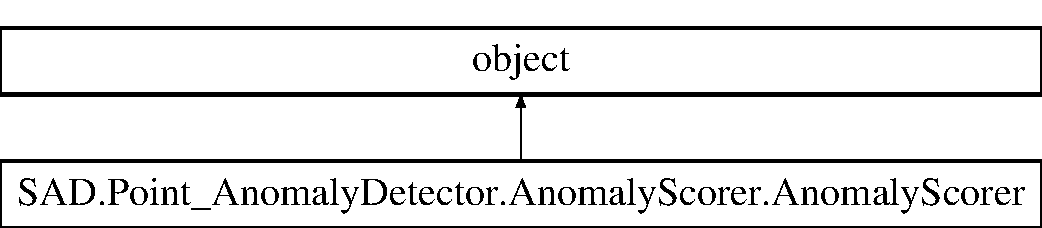
\includegraphics[height=2.000000cm]{classSAD_1_1Point__AnomalyDetector_1_1AnomalyScorer_1_1AnomalyScorer}
\end{center}
\end{figure}
\subsection*{Public Member Functions}
\begin{DoxyCompactItemize}
\item 
def \hyperlink{classSAD_1_1Point__AnomalyDetector_1_1AnomalyScorer_1_1AnomalyScorer_a4109f8186ad1aa9c28c2f12fcc36c714}{\+\_\+\+\_\+init\+\_\+\+\_\+} (self)
\item 
def \hyperlink{classSAD_1_1Point__AnomalyDetector_1_1AnomalyScorer_1_1AnomalyScorer_a22e40f7116e20bd61b81510970266151}{Train\+\_\+\+Point\+Detector} (self, data=\mbox{[}$\,$\mbox{]})
\end{DoxyCompactItemize}


\subsection{Constructor \& Destructor Documentation}
\index{S\+A\+D\+::\+Point\+\_\+\+Anomaly\+Detector\+::\+Anomaly\+Scorer\+::\+Anomaly\+Scorer@{S\+A\+D\+::\+Point\+\_\+\+Anomaly\+Detector\+::\+Anomaly\+Scorer\+::\+Anomaly\+Scorer}!\+\_\+\+\_\+init\+\_\+\+\_\+@{\+\_\+\+\_\+init\+\_\+\+\_\+}}
\index{\+\_\+\+\_\+init\+\_\+\+\_\+@{\+\_\+\+\_\+init\+\_\+\+\_\+}!S\+A\+D\+::\+Point\+\_\+\+Anomaly\+Detector\+::\+Anomaly\+Scorer\+::\+Anomaly\+Scorer@{S\+A\+D\+::\+Point\+\_\+\+Anomaly\+Detector\+::\+Anomaly\+Scorer\+::\+Anomaly\+Scorer}}
\subsubsection[{\texorpdfstring{\+\_\+\+\_\+init\+\_\+\+\_\+(self)}{__init__(self)}}]{\setlength{\rightskip}{0pt plus 5cm}def S\+A\+D.\+Point\+\_\+\+Anomaly\+Detector.\+Anomaly\+Scorer.\+Anomaly\+Scorer.\+\_\+\+\_\+init\+\_\+\+\_\+ (
\begin{DoxyParamCaption}
\item[{}]{self}
\end{DoxyParamCaption}
)}\hypertarget{classSAD_1_1Point__AnomalyDetector_1_1AnomalyScorer_1_1AnomalyScorer_a4109f8186ad1aa9c28c2f12fcc36c714}{}\label{classSAD_1_1Point__AnomalyDetector_1_1AnomalyScorer_1_1AnomalyScorer_a4109f8186ad1aa9c28c2f12fcc36c714}
\begin{DoxyVerb}This is the super class for the point anomaly detector
:return:
\end{DoxyVerb}
 

\subsection{Member Function Documentation}
\index{S\+A\+D\+::\+Point\+\_\+\+Anomaly\+Detector\+::\+Anomaly\+Scorer\+::\+Anomaly\+Scorer@{S\+A\+D\+::\+Point\+\_\+\+Anomaly\+Detector\+::\+Anomaly\+Scorer\+::\+Anomaly\+Scorer}!Train\+\_\+\+Point\+Detector@{Train\+\_\+\+Point\+Detector}}
\index{Train\+\_\+\+Point\+Detector@{Train\+\_\+\+Point\+Detector}!S\+A\+D\+::\+Point\+\_\+\+Anomaly\+Detector\+::\+Anomaly\+Scorer\+::\+Anomaly\+Scorer@{S\+A\+D\+::\+Point\+\_\+\+Anomaly\+Detector\+::\+Anomaly\+Scorer\+::\+Anomaly\+Scorer}}
\subsubsection[{\texorpdfstring{Train\+\_\+\+Point\+Detector(self, data=[])}{Train_PointDetector(self, data=[])}}]{\setlength{\rightskip}{0pt plus 5cm}def S\+A\+D.\+Point\+\_\+\+Anomaly\+Detector.\+Anomaly\+Scorer.\+Anomaly\+Scorer.\+Train\+\_\+\+Point\+Detector (
\begin{DoxyParamCaption}
\item[{}]{self, }
\item[{}]{data = {\ttfamily \mbox{[}\mbox{]}}}
\end{DoxyParamCaption}
)}\hypertarget{classSAD_1_1Point__AnomalyDetector_1_1AnomalyScorer_1_1AnomalyScorer_a22e40f7116e20bd61b81510970266151}{}\label{classSAD_1_1Point__AnomalyDetector_1_1AnomalyScorer_1_1AnomalyScorer_a22e40f7116e20bd61b81510970266151}
\begin{DoxyVerb}:param data:train the point detector according to the data
:return:
\end{DoxyVerb}
 

The documentation for this class was generated from the following file\+:\begin{DoxyCompactItemize}
\item 
Point\+\_\+\+Anomaly\+Detector/Anomaly\+Scorer.\+py\end{DoxyCompactItemize}

\hypertarget{classSAD_1_1Stream__AnomalyDetector_1_1CUSUM_1_1CUSUM}{}\section{S\+A\+D.\+Stream\+\_\+\+Anomaly\+Detector.\+C\+U\+S\+U\+M.\+C\+U\+S\+UM Class Reference}
\label{classSAD_1_1Stream__AnomalyDetector_1_1CUSUM_1_1CUSUM}\index{S\+A\+D.\+Stream\+\_\+\+Anomaly\+Detector.\+C\+U\+S\+U\+M.\+C\+U\+S\+UM@{S\+A\+D.\+Stream\+\_\+\+Anomaly\+Detector.\+C\+U\+S\+U\+M.\+C\+U\+S\+UM}}
Inheritance diagram for S\+A\+D.\+Stream\+\_\+\+Anomaly\+Detector.\+C\+U\+S\+U\+M.\+C\+U\+S\+UM\+:\begin{figure}[H]
\begin{center}
\leavevmode
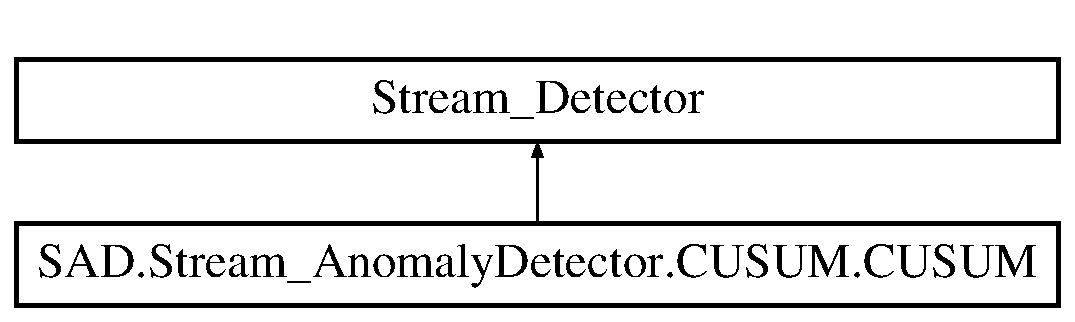
\includegraphics[height=2.000000cm]{classSAD_1_1Stream__AnomalyDetector_1_1CUSUM_1_1CUSUM}
\end{center}
\end{figure}
\subsection*{Public Member Functions}
\begin{DoxyCompactItemize}
\item 
def \hyperlink{classSAD_1_1Stream__AnomalyDetector_1_1CUSUM_1_1CUSUM_aea65fbf9e16b126dad9c1b91fe734a30}{\+\_\+\+\_\+init\+\_\+\+\_\+} (self, drift=1, threshold=1)
\item 
def \hyperlink{classSAD_1_1Stream__AnomalyDetector_1_1CUSUM_1_1CUSUM_a54cc2ba467941bf9413936ee882f456d}{check} (self, score)
\end{DoxyCompactItemize}
\subsection*{Public Attributes}
\begin{DoxyCompactItemize}
\item 
{\bfseries Detector}\hypertarget{classSAD_1_1Stream__AnomalyDetector_1_1CUSUM_1_1CUSUM_a323dd6bb57c96d09d2435fba0541503e}{}\label{classSAD_1_1Stream__AnomalyDetector_1_1CUSUM_1_1CUSUM_a323dd6bb57c96d09d2435fba0541503e}

\end{DoxyCompactItemize}


\subsection{Constructor \& Destructor Documentation}
\index{S\+A\+D\+::\+Stream\+\_\+\+Anomaly\+Detector\+::\+C\+U\+S\+U\+M\+::\+C\+U\+S\+UM@{S\+A\+D\+::\+Stream\+\_\+\+Anomaly\+Detector\+::\+C\+U\+S\+U\+M\+::\+C\+U\+S\+UM}!\+\_\+\+\_\+init\+\_\+\+\_\+@{\+\_\+\+\_\+init\+\_\+\+\_\+}}
\index{\+\_\+\+\_\+init\+\_\+\+\_\+@{\+\_\+\+\_\+init\+\_\+\+\_\+}!S\+A\+D\+::\+Stream\+\_\+\+Anomaly\+Detector\+::\+C\+U\+S\+U\+M\+::\+C\+U\+S\+UM@{S\+A\+D\+::\+Stream\+\_\+\+Anomaly\+Detector\+::\+C\+U\+S\+U\+M\+::\+C\+U\+S\+UM}}
\subsubsection[{\texorpdfstring{\+\_\+\+\_\+init\+\_\+\+\_\+(self, drift=1, threshold=1)}{__init__(self, drift=1, threshold=1)}}]{\setlength{\rightskip}{0pt plus 5cm}def S\+A\+D.\+Stream\+\_\+\+Anomaly\+Detector.\+C\+U\+S\+U\+M.\+C\+U\+S\+U\+M.\+\_\+\+\_\+init\+\_\+\+\_\+ (
\begin{DoxyParamCaption}
\item[{}]{self, }
\item[{}]{drift = {\ttfamily 1}, }
\item[{}]{threshold = {\ttfamily 1}}
\end{DoxyParamCaption}
)}\hypertarget{classSAD_1_1Stream__AnomalyDetector_1_1CUSUM_1_1CUSUM_aea65fbf9e16b126dad9c1b91fe734a30}{}\label{classSAD_1_1Stream__AnomalyDetector_1_1CUSUM_1_1CUSUM_aea65fbf9e16b126dad9c1b91fe734a30}
\begin{DoxyVerb}This the stream detector using CUSUM algorithm
:param drift: The drift of the score that could be detected
:param threshold: the threshold that during some period the positive and negative changes exceeds the threshold
:return:
\end{DoxyVerb}
 

\subsection{Member Function Documentation}
\index{S\+A\+D\+::\+Stream\+\_\+\+Anomaly\+Detector\+::\+C\+U\+S\+U\+M\+::\+C\+U\+S\+UM@{S\+A\+D\+::\+Stream\+\_\+\+Anomaly\+Detector\+::\+C\+U\+S\+U\+M\+::\+C\+U\+S\+UM}!check@{check}}
\index{check@{check}!S\+A\+D\+::\+Stream\+\_\+\+Anomaly\+Detector\+::\+C\+U\+S\+U\+M\+::\+C\+U\+S\+UM@{S\+A\+D\+::\+Stream\+\_\+\+Anomaly\+Detector\+::\+C\+U\+S\+U\+M\+::\+C\+U\+S\+UM}}
\subsubsection[{\texorpdfstring{check(self, score)}{check(self, score)}}]{\setlength{\rightskip}{0pt plus 5cm}def S\+A\+D.\+Stream\+\_\+\+Anomaly\+Detector.\+C\+U\+S\+U\+M.\+C\+U\+S\+U\+M.\+check (
\begin{DoxyParamCaption}
\item[{}]{self, }
\item[{}]{score}
\end{DoxyParamCaption}
)}\hypertarget{classSAD_1_1Stream__AnomalyDetector_1_1CUSUM_1_1CUSUM_a54cc2ba467941bf9413936ee882f456d}{}\label{classSAD_1_1Stream__AnomalyDetector_1_1CUSUM_1_1CUSUM_a54cc2ba467941bf9413936ee882f456d}
\begin{DoxyVerb}Check whether an anomalous happens for the incoming score
:param score: The incoming score
:return: Whether a drift detected
\end{DoxyVerb}
 

The documentation for this class was generated from the following file\+:\begin{DoxyCompactItemize}
\item 
Stream\+\_\+\+Anomaly\+Detector/C\+U\+S\+U\+M.\+py\end{DoxyCompactItemize}

\hypertarget{classSAD_1_1Stream__Generator_1_1Dataset__Generator_1_1Dataset__Generator}{}\section{S\+A\+D.\+Stream\+\_\+\+Generator.\+Dataset\+\_\+\+Generator.\+Dataset\+\_\+\+Generator Class Reference}
\label{classSAD_1_1Stream__Generator_1_1Dataset__Generator_1_1Dataset__Generator}\index{S\+A\+D.\+Stream\+\_\+\+Generator.\+Dataset\+\_\+\+Generator.\+Dataset\+\_\+\+Generator@{S\+A\+D.\+Stream\+\_\+\+Generator.\+Dataset\+\_\+\+Generator.\+Dataset\+\_\+\+Generator}}


Inheritance diagram for S\+A\+D.\+Stream\+\_\+\+Generator.\+Dataset\+\_\+\+Generator.\+Dataset\+\_\+\+Generator\+:\nopagebreak
\begin{figure}[H]
\begin{center}
\leavevmode
\includegraphics[width=236pt]{classSAD_1_1Stream__Generator_1_1Dataset__Generator_1_1Dataset__Generator__inherit__graph}
\end{center}
\end{figure}


Collaboration diagram for S\+A\+D.\+Stream\+\_\+\+Generator.\+Dataset\+\_\+\+Generator.\+Dataset\+\_\+\+Generator\+:\nopagebreak
\begin{figure}[H]
\begin{center}
\leavevmode
\includegraphics[width=236pt]{classSAD_1_1Stream__Generator_1_1Dataset__Generator_1_1Dataset__Generator__coll__graph}
\end{center}
\end{figure}
\subsection*{Public Member Functions}
\begin{DoxyCompactItemize}
\item 
def \hyperlink{classSAD_1_1Stream__Generator_1_1Dataset__Generator_1_1Dataset__Generator_a96fe8d29f2e2d15797d6ed779df19648}{\+\_\+\+\_\+init\+\_\+\+\_\+} (self, filename, delimiter=\char`\"{},  normal\+\_\+class=\char`\"{}value\char`\"{},  column=-\/1,  type\+\_\+error=\char`\"{}Sudden\char`\"{})
\item 
def \hyperlink{classSAD_1_1Stream__Generator_1_1Dataset__Generator_1_1Dataset__Generator_ab370a4bfa53c33a13085cae10de52a5a}{Generate\+\_\+\+Train\+Data} (self, percentage)
\item 
def \hyperlink{classSAD_1_1Stream__Generator_1_1Dataset__Generator_1_1Dataset__Generator_a168344d3d081678884e42083cc0ef033}{Generate\+\_\+\+Stream} (self, type, number)
\end{DoxyCompactItemize}
\subsection*{Public Attributes}
\begin{DoxyCompactItemize}
\item 
{\bfseries attribute}\hypertarget{classSAD_1_1Stream__Generator_1_1Dataset__Generator_1_1Dataset__Generator_ae797910a2d2eccde0a4e7b7532e70efd}{}\label{classSAD_1_1Stream__Generator_1_1Dataset__Generator_1_1Dataset__Generator_ae797910a2d2eccde0a4e7b7532e70efd}

\item 
{\bfseries Normal\+\_\+data\+\_\+set}\hypertarget{classSAD_1_1Stream__Generator_1_1Dataset__Generator_1_1Dataset__Generator_a1227628193348bedbff73702c2feb623}{}\label{classSAD_1_1Stream__Generator_1_1Dataset__Generator_1_1Dataset__Generator_a1227628193348bedbff73702c2feb623}

\item 
{\bfseries Anormal\+\_\+data\+\_\+set}\hypertarget{classSAD_1_1Stream__Generator_1_1Dataset__Generator_1_1Dataset__Generator_a60eeb9eb166ef7a13c71bf1aba7ce9a1}{}\label{classSAD_1_1Stream__Generator_1_1Dataset__Generator_1_1Dataset__Generator_a60eeb9eb166ef7a13c71bf1aba7ce9a1}

\item 
{\bfseries train}\hypertarget{classSAD_1_1Stream__Generator_1_1Dataset__Generator_1_1Dataset__Generator_aede62d4b644010a0f45b0f633c3fc88c}{}\label{classSAD_1_1Stream__Generator_1_1Dataset__Generator_1_1Dataset__Generator_aede62d4b644010a0f45b0f633c3fc88c}

\item 
{\bfseries test}\hypertarget{classSAD_1_1Stream__Generator_1_1Dataset__Generator_1_1Dataset__Generator_af99150065cc9eea9d2b4a10f31138b4d}{}\label{classSAD_1_1Stream__Generator_1_1Dataset__Generator_1_1Dataset__Generator_af99150065cc9eea9d2b4a10f31138b4d}

\item 
{\bfseries type\+\_\+error}\hypertarget{classSAD_1_1Stream__Generator_1_1Dataset__Generator_1_1Dataset__Generator_a35016c0d5eb7228b837c9e1913d40c50}{}\label{classSAD_1_1Stream__Generator_1_1Dataset__Generator_1_1Dataset__Generator_a35016c0d5eb7228b837c9e1913d40c50}

\end{DoxyCompactItemize}


\subsection{Constructor \& Destructor Documentation}
\index{S\+A\+D\+::\+Stream\+\_\+\+Generator\+::\+Dataset\+\_\+\+Generator\+::\+Dataset\+\_\+\+Generator@{S\+A\+D\+::\+Stream\+\_\+\+Generator\+::\+Dataset\+\_\+\+Generator\+::\+Dataset\+\_\+\+Generator}!\+\_\+\+\_\+init\+\_\+\+\_\+@{\+\_\+\+\_\+init\+\_\+\+\_\+}}
\index{\+\_\+\+\_\+init\+\_\+\+\_\+@{\+\_\+\+\_\+init\+\_\+\+\_\+}!S\+A\+D\+::\+Stream\+\_\+\+Generator\+::\+Dataset\+\_\+\+Generator\+::\+Dataset\+\_\+\+Generator@{S\+A\+D\+::\+Stream\+\_\+\+Generator\+::\+Dataset\+\_\+\+Generator\+::\+Dataset\+\_\+\+Generator}}
\subsubsection[{\texorpdfstring{\+\_\+\+\_\+init\+\_\+\+\_\+(self, filename, delimiter="",  normal\+\_\+class=""value"",  column=-\/1,  type\+\_\+error=""Sudden"")}{__init__(self, filename, delimiter=",  normal_class="value",  column=-1,  type_error="Sudden")}}]{\setlength{\rightskip}{0pt plus 5cm}def S\+A\+D.\+Stream\+\_\+\+Generator.\+Dataset\+\_\+\+Generator.\+Dataset\+\_\+\+Generator.\+\_\+\+\_\+init\+\_\+\+\_\+ (
\begin{DoxyParamCaption}
\item[{}]{self, }
\item[{}]{filename, }
\item[{}]{delimiter = {\ttfamily \char`\"{}}, }
\item[{}]{normal\+\_\+class = {\ttfamily \char`\"{}value\char`\"{}}, }
\item[{}]{column = {\ttfamily -\/1}, }
\item[{}]{type\+\_\+error = {\ttfamily \char`\"{}Sudden\char`\"{}}}
\end{DoxyParamCaption}
)}\hypertarget{classSAD_1_1Stream__Generator_1_1Dataset__Generator_1_1Dataset__Generator_a96fe8d29f2e2d15797d6ed779df19648}{}\label{classSAD_1_1Stream__Generator_1_1Dataset__Generator_1_1Dataset__Generator_a96fe8d29f2e2d15797d6ed779df19648}
\begin{DoxyVerb}For generating the stream data from data_set
If the need training phase, also used for generating train_data
For stream data, they could generate errors from type_error
:param filename: the filename for the data set
:param delimiter: the delimiter in the data set
:param normal_class: the normal class of the data set
:param column: the column for the feature
:param type_error: the type of the error
:return:
\end{DoxyVerb}
 

\subsection{Member Function Documentation}
\index{S\+A\+D\+::\+Stream\+\_\+\+Generator\+::\+Dataset\+\_\+\+Generator\+::\+Dataset\+\_\+\+Generator@{S\+A\+D\+::\+Stream\+\_\+\+Generator\+::\+Dataset\+\_\+\+Generator\+::\+Dataset\+\_\+\+Generator}!Generate\+\_\+\+Stream@{Generate\+\_\+\+Stream}}
\index{Generate\+\_\+\+Stream@{Generate\+\_\+\+Stream}!S\+A\+D\+::\+Stream\+\_\+\+Generator\+::\+Dataset\+\_\+\+Generator\+::\+Dataset\+\_\+\+Generator@{S\+A\+D\+::\+Stream\+\_\+\+Generator\+::\+Dataset\+\_\+\+Generator\+::\+Dataset\+\_\+\+Generator}}
\subsubsection[{\texorpdfstring{Generate\+\_\+\+Stream(self, type, number)}{Generate_Stream(self, type, number)}}]{\setlength{\rightskip}{0pt plus 5cm}def S\+A\+D.\+Stream\+\_\+\+Generator.\+Dataset\+\_\+\+Generator.\+Dataset\+\_\+\+Generator.\+Generate\+\_\+\+Stream (
\begin{DoxyParamCaption}
\item[{}]{self, }
\item[{}]{type, }
\item[{}]{number}
\end{DoxyParamCaption}
)}\hypertarget{classSAD_1_1Stream__Generator_1_1Dataset__Generator_1_1Dataset__Generator_a168344d3d081678884e42083cc0ef033}{}\label{classSAD_1_1Stream__Generator_1_1Dataset__Generator_1_1Dataset__Generator_a168344d3d081678884e42083cc0ef033}
\begin{DoxyVerb}:param type: type is either normal or anomaly
:param number: number of the stream data generated
:return: the matrix of the stream data according to the distribution and type
\end{DoxyVerb}
 \index{S\+A\+D\+::\+Stream\+\_\+\+Generator\+::\+Dataset\+\_\+\+Generator\+::\+Dataset\+\_\+\+Generator@{S\+A\+D\+::\+Stream\+\_\+\+Generator\+::\+Dataset\+\_\+\+Generator\+::\+Dataset\+\_\+\+Generator}!Generate\+\_\+\+Train\+Data@{Generate\+\_\+\+Train\+Data}}
\index{Generate\+\_\+\+Train\+Data@{Generate\+\_\+\+Train\+Data}!S\+A\+D\+::\+Stream\+\_\+\+Generator\+::\+Dataset\+\_\+\+Generator\+::\+Dataset\+\_\+\+Generator@{S\+A\+D\+::\+Stream\+\_\+\+Generator\+::\+Dataset\+\_\+\+Generator\+::\+Dataset\+\_\+\+Generator}}
\subsubsection[{\texorpdfstring{Generate\+\_\+\+Train\+Data(self, percentage)}{Generate_TrainData(self, percentage)}}]{\setlength{\rightskip}{0pt plus 5cm}def S\+A\+D.\+Stream\+\_\+\+Generator.\+Dataset\+\_\+\+Generator.\+Dataset\+\_\+\+Generator.\+Generate\+\_\+\+Train\+Data (
\begin{DoxyParamCaption}
\item[{}]{self, }
\item[{}]{percentage}
\end{DoxyParamCaption}
)}\hypertarget{classSAD_1_1Stream__Generator_1_1Dataset__Generator_1_1Dataset__Generator_ab370a4bfa53c33a13085cae10de52a5a}{}\label{classSAD_1_1Stream__Generator_1_1Dataset__Generator_1_1Dataset__Generator_ab370a4bfa53c33a13085cae10de52a5a}
\begin{DoxyVerb}:param percentage: if in not incremental mode, the percentage is the training percentage
:return:
\end{DoxyVerb}
 

The documentation for this class was generated from the following file\+:\begin{DoxyCompactItemize}
\item 
Stream\+\_\+\+Generator/Dataset\+\_\+\+Generator.\+py\end{DoxyCompactItemize}

\hypertarget{classSAD_1_1Stream__AnomalyDetector_1_1DDM_1_1DDM}{}\section{S\+A\+D.\+Stream\+\_\+\+Anomaly\+Detector.\+D\+D\+M.\+D\+DM Class Reference}
\label{classSAD_1_1Stream__AnomalyDetector_1_1DDM_1_1DDM}\index{S\+A\+D.\+Stream\+\_\+\+Anomaly\+Detector.\+D\+D\+M.\+D\+DM@{S\+A\+D.\+Stream\+\_\+\+Anomaly\+Detector.\+D\+D\+M.\+D\+DM}}


Inheritance diagram for S\+A\+D.\+Stream\+\_\+\+Anomaly\+Detector.\+D\+D\+M.\+D\+DM\+:\nopagebreak
\begin{figure}[H]
\begin{center}
\leavevmode
\includegraphics[width=236pt]{classSAD_1_1Stream__AnomalyDetector_1_1DDM_1_1DDM__inherit__graph}
\end{center}
\end{figure}


Collaboration diagram for S\+A\+D.\+Stream\+\_\+\+Anomaly\+Detector.\+D\+D\+M.\+D\+DM\+:\nopagebreak
\begin{figure}[H]
\begin{center}
\leavevmode
\includegraphics[width=236pt]{classSAD_1_1Stream__AnomalyDetector_1_1DDM_1_1DDM__coll__graph}
\end{center}
\end{figure}
\subsection*{Public Member Functions}
\begin{DoxyCompactItemize}
\item 
def \hyperlink{classSAD_1_1Stream__AnomalyDetector_1_1DDM_1_1DDM_a1cb03342401690d45ffa9e7981d37d38}{\+\_\+\+\_\+init\+\_\+\+\_\+} (self, threshold=1, alpha=2.\+0, beta=3.\+0)
\item 
def \hyperlink{classSAD_1_1Stream__AnomalyDetector_1_1DDM_1_1DDM_ae2afdf68bb18604f54496559f3d3577a}{check} (self, score)
\end{DoxyCompactItemize}
\subsection*{Public Attributes}
\begin{DoxyCompactItemize}
\item 
{\bfseries Detector}\hypertarget{classSAD_1_1Stream__AnomalyDetector_1_1DDM_1_1DDM_acf042d7d556742c3573344d08539ab95}{}\label{classSAD_1_1Stream__AnomalyDetector_1_1DDM_1_1DDM_acf042d7d556742c3573344d08539ab95}

\end{DoxyCompactItemize}


\subsection{Constructor \& Destructor Documentation}
\index{S\+A\+D\+::\+Stream\+\_\+\+Anomaly\+Detector\+::\+D\+D\+M\+::\+D\+DM@{S\+A\+D\+::\+Stream\+\_\+\+Anomaly\+Detector\+::\+D\+D\+M\+::\+D\+DM}!\+\_\+\+\_\+init\+\_\+\+\_\+@{\+\_\+\+\_\+init\+\_\+\+\_\+}}
\index{\+\_\+\+\_\+init\+\_\+\+\_\+@{\+\_\+\+\_\+init\+\_\+\+\_\+}!S\+A\+D\+::\+Stream\+\_\+\+Anomaly\+Detector\+::\+D\+D\+M\+::\+D\+DM@{S\+A\+D\+::\+Stream\+\_\+\+Anomaly\+Detector\+::\+D\+D\+M\+::\+D\+DM}}
\subsubsection[{\texorpdfstring{\+\_\+\+\_\+init\+\_\+\+\_\+(self, threshold=1, alpha=2.\+0, beta=3.\+0)}{__init__(self, threshold=1, alpha=2.0, beta=3.0)}}]{\setlength{\rightskip}{0pt plus 5cm}def S\+A\+D.\+Stream\+\_\+\+Anomaly\+Detector.\+D\+D\+M.\+D\+D\+M.\+\_\+\+\_\+init\+\_\+\+\_\+ (
\begin{DoxyParamCaption}
\item[{}]{self, }
\item[{}]{threshold = {\ttfamily 1}, }
\item[{}]{alpha = {\ttfamily 2.0}, }
\item[{}]{beta = {\ttfamily 3.0}}
\end{DoxyParamCaption}
)}\hypertarget{classSAD_1_1Stream__AnomalyDetector_1_1DDM_1_1DDM_a1cb03342401690d45ffa9e7981d37d38}{}\label{classSAD_1_1Stream__AnomalyDetector_1_1DDM_1_1DDM_a1cb03342401690d45ffa9e7981d37d38}
\begin{DoxyVerb}This is the stream detector using DDM algorithm
:param threshold: When the score exceeds the threshold then the prob of anomalous increases
:return:
\end{DoxyVerb}
 

\subsection{Member Function Documentation}
\index{S\+A\+D\+::\+Stream\+\_\+\+Anomaly\+Detector\+::\+D\+D\+M\+::\+D\+DM@{S\+A\+D\+::\+Stream\+\_\+\+Anomaly\+Detector\+::\+D\+D\+M\+::\+D\+DM}!check@{check}}
\index{check@{check}!S\+A\+D\+::\+Stream\+\_\+\+Anomaly\+Detector\+::\+D\+D\+M\+::\+D\+DM@{S\+A\+D\+::\+Stream\+\_\+\+Anomaly\+Detector\+::\+D\+D\+M\+::\+D\+DM}}
\subsubsection[{\texorpdfstring{check(self, score)}{check(self, score)}}]{\setlength{\rightskip}{0pt plus 5cm}def S\+A\+D.\+Stream\+\_\+\+Anomaly\+Detector.\+D\+D\+M.\+D\+D\+M.\+check (
\begin{DoxyParamCaption}
\item[{}]{self, }
\item[{}]{score}
\end{DoxyParamCaption}
)}\hypertarget{classSAD_1_1Stream__AnomalyDetector_1_1DDM_1_1DDM_ae2afdf68bb18604f54496559f3d3577a}{}\label{classSAD_1_1Stream__AnomalyDetector_1_1DDM_1_1DDM_ae2afdf68bb18604f54496559f3d3577a}
\begin{DoxyVerb}Check whether an anomalous happens for the incoming score
:param score: The incoming score
:return: Whether a drift detected
\end{DoxyVerb}
 

The documentation for this class was generated from the following file\+:\begin{DoxyCompactItemize}
\item 
Stream\+\_\+\+Anomaly\+Detector/D\+D\+M.\+py\end{DoxyCompactItemize}

\input{classSAD_1_1Stream__AnomalyDetector_1_1FCWM_1_1FCWM}
\hypertarget{classSAD_1_1Point__AnomalyDetector_1_1Fit__data_1_1Fit__data}{}\section{S\+A\+D.\+Point\+\_\+\+Anomaly\+Detector.\+Fit\+\_\+data.\+Fit\+\_\+data Class Reference}
\label{classSAD_1_1Point__AnomalyDetector_1_1Fit__data_1_1Fit__data}\index{S\+A\+D.\+Point\+\_\+\+Anomaly\+Detector.\+Fit\+\_\+data.\+Fit\+\_\+data@{S\+A\+D.\+Point\+\_\+\+Anomaly\+Detector.\+Fit\+\_\+data.\+Fit\+\_\+data}}
\subsection*{Public Member Functions}
\begin{DoxyCompactItemize}
\item 
def \hyperlink{classSAD_1_1Point__AnomalyDetector_1_1Fit__data_1_1Fit__data_aa5728a908c85eb5d012d9e6452280897}{find\+\_\+distribution} (self, data, test\+\_\+distribution=\mbox{[}\textquotesingle{}norm\textquotesingle{}\mbox{]})
\end{DoxyCompactItemize}


\subsection{Member Function Documentation}
\index{S\+A\+D\+::\+Point\+\_\+\+Anomaly\+Detector\+::\+Fit\+\_\+data\+::\+Fit\+\_\+data@{S\+A\+D\+::\+Point\+\_\+\+Anomaly\+Detector\+::\+Fit\+\_\+data\+::\+Fit\+\_\+data}!find\+\_\+distribution@{find\+\_\+distribution}}
\index{find\+\_\+distribution@{find\+\_\+distribution}!S\+A\+D\+::\+Point\+\_\+\+Anomaly\+Detector\+::\+Fit\+\_\+data\+::\+Fit\+\_\+data@{S\+A\+D\+::\+Point\+\_\+\+Anomaly\+Detector\+::\+Fit\+\_\+data\+::\+Fit\+\_\+data}}
\subsubsection[{\texorpdfstring{find\+\_\+distribution(self, data, test\+\_\+distribution=[\textquotesingle{}norm\textquotesingle{}])}{find_distribution(self, data, test_distribution=['norm'])}}]{\setlength{\rightskip}{0pt plus 5cm}def S\+A\+D.\+Point\+\_\+\+Anomaly\+Detector.\+Fit\+\_\+data.\+Fit\+\_\+data.\+find\+\_\+distribution (
\begin{DoxyParamCaption}
\item[{}]{self, }
\item[{}]{data, }
\item[{}]{test\+\_\+distribution = {\ttfamily \mbox{[}\textquotesingle{}norm\textquotesingle{}\mbox{]}}}
\end{DoxyParamCaption}
)}\hypertarget{classSAD_1_1Point__AnomalyDetector_1_1Fit__data_1_1Fit__data_aa5728a908c85eb5d012d9e6452280897}{}\label{classSAD_1_1Point__AnomalyDetector_1_1Fit__data_1_1Fit__data_aa5728a908c85eb5d012d9e6452280897}
\begin{DoxyVerb}This is for finding the suitable distribution from test_distributions and poisson
use the package of fitter
:param data: The data which wants to be trained
:param test_distribution: the lists of the distributions which will be used in _fit_continuous
:return:
\end{DoxyVerb}
 

The documentation for this class was generated from the following file\+:\begin{DoxyCompactItemize}
\item 
Point\+\_\+\+Anomaly\+Detector/Fit\+\_\+data.\+py\end{DoxyCompactItemize}

\hypertarget{classSAD_1_1Stream__Generator_1_1Generator_1_1Generator}{}\section{S\+A\+D.\+Stream\+\_\+\+Generator.\+Generator.\+Generator Class Reference}
\label{classSAD_1_1Stream__Generator_1_1Generator_1_1Generator}\index{S\+A\+D.\+Stream\+\_\+\+Generator.\+Generator.\+Generator@{S\+A\+D.\+Stream\+\_\+\+Generator.\+Generator.\+Generator}}


Inheritance diagram for S\+A\+D.\+Stream\+\_\+\+Generator.\+Generator.\+Generator\+:\nopagebreak
\begin{figure}[H]
\begin{center}
\leavevmode
\includegraphics[width=248pt]{classSAD_1_1Stream__Generator_1_1Generator_1_1Generator__inherit__graph}
\end{center}
\end{figure}


Collaboration diagram for S\+A\+D.\+Stream\+\_\+\+Generator.\+Generator.\+Generator\+:\nopagebreak
\begin{figure}[H]
\begin{center}
\leavevmode
\includegraphics[width=248pt]{classSAD_1_1Stream__Generator_1_1Generator_1_1Generator__coll__graph}
\end{center}
\end{figure}
\subsection*{Public Member Functions}
\begin{DoxyCompactItemize}
\item 
def \hyperlink{classSAD_1_1Stream__Generator_1_1Generator_1_1Generator_a5377eee3255f592c8784613ec36d9b7b}{\+\_\+\+\_\+init\+\_\+\+\_\+} (self, type\+\_\+error=\char`\"{}Sudden\char`\"{})
\item 
def \hyperlink{classSAD_1_1Stream__Generator_1_1Generator_1_1Generator_a7f0553ca2a50b0f9e840b0348a3b47ee}{Generate\+\_\+\+Train\+Data} (self)
\item 
def \hyperlink{classSAD_1_1Stream__Generator_1_1Generator_1_1Generator_a6baa6039a6203f9be7b10ddf4ec44775}{Generate\+\_\+\+Stream} (self, type=\char`\"{}Normal\char`\"{}, number=0)
\end{DoxyCompactItemize}
\subsection*{Public Attributes}
\begin{DoxyCompactItemize}
\item 
{\bfseries Myseed}\hypertarget{classSAD_1_1Stream__Generator_1_1Generator_1_1Generator_a568e3ac6061922513adca4061782dc01}{}\label{classSAD_1_1Stream__Generator_1_1Generator_1_1Generator_a568e3ac6061922513adca4061782dc01}

\item 
{\bfseries ran}\hypertarget{classSAD_1_1Stream__Generator_1_1Generator_1_1Generator_adde13947a474859765e81bb51aa9d9cb}{}\label{classSAD_1_1Stream__Generator_1_1Generator_1_1Generator_adde13947a474859765e81bb51aa9d9cb}

\item 
{\bfseries type\+\_\+error}\hypertarget{classSAD_1_1Stream__Generator_1_1Generator_1_1Generator_a9750f7a437158be00b9421d92103b4c9}{}\label{classSAD_1_1Stream__Generator_1_1Generator_1_1Generator_a9750f7a437158be00b9421d92103b4c9}

\end{DoxyCompactItemize}


\subsection{Constructor \& Destructor Documentation}
\index{S\+A\+D\+::\+Stream\+\_\+\+Generator\+::\+Generator\+::\+Generator@{S\+A\+D\+::\+Stream\+\_\+\+Generator\+::\+Generator\+::\+Generator}!\+\_\+\+\_\+init\+\_\+\+\_\+@{\+\_\+\+\_\+init\+\_\+\+\_\+}}
\index{\+\_\+\+\_\+init\+\_\+\+\_\+@{\+\_\+\+\_\+init\+\_\+\+\_\+}!S\+A\+D\+::\+Stream\+\_\+\+Generator\+::\+Generator\+::\+Generator@{S\+A\+D\+::\+Stream\+\_\+\+Generator\+::\+Generator\+::\+Generator}}
\subsubsection[{\texorpdfstring{\+\_\+\+\_\+init\+\_\+\+\_\+(self, type\+\_\+error=""Sudden"")}{__init__(self, type_error="Sudden")}}]{\setlength{\rightskip}{0pt plus 5cm}def S\+A\+D.\+Stream\+\_\+\+Generator.\+Generator.\+Generator.\+\_\+\+\_\+init\+\_\+\+\_\+ (
\begin{DoxyParamCaption}
\item[{}]{self, }
\item[{}]{type\+\_\+error = {\ttfamily \char`\"{}Sudden\char`\"{}}}
\end{DoxyParamCaption}
)}\hypertarget{classSAD_1_1Stream__Generator_1_1Generator_1_1Generator_a5377eee3255f592c8784613ec36d9b7b}{}\label{classSAD_1_1Stream__Generator_1_1Generator_1_1Generator_a5377eee3255f592c8784613ec36d9b7b}
\begin{DoxyVerb}The super class of the Generator
:param type_error:Type of the errors generated in the simulation and datastamp data, it's not useful for the timestamp
:return:
\end{DoxyVerb}
 

\subsection{Member Function Documentation}
\index{S\+A\+D\+::\+Stream\+\_\+\+Generator\+::\+Generator\+::\+Generator@{S\+A\+D\+::\+Stream\+\_\+\+Generator\+::\+Generator\+::\+Generator}!Generate\+\_\+\+Stream@{Generate\+\_\+\+Stream}}
\index{Generate\+\_\+\+Stream@{Generate\+\_\+\+Stream}!S\+A\+D\+::\+Stream\+\_\+\+Generator\+::\+Generator\+::\+Generator@{S\+A\+D\+::\+Stream\+\_\+\+Generator\+::\+Generator\+::\+Generator}}
\subsubsection[{\texorpdfstring{Generate\+\_\+\+Stream(self, type=""Normal"", number=0)}{Generate_Stream(self, type="Normal", number=0)}}]{\setlength{\rightskip}{0pt plus 5cm}def S\+A\+D.\+Stream\+\_\+\+Generator.\+Generator.\+Generator.\+Generate\+\_\+\+Stream (
\begin{DoxyParamCaption}
\item[{}]{self, }
\item[{}]{type = {\ttfamily \char`\"{}Normal\char`\"{}}, }
\item[{}]{number = {\ttfamily 0}}
\end{DoxyParamCaption}
)}\hypertarget{classSAD_1_1Stream__Generator_1_1Generator_1_1Generator_a6baa6039a6203f9be7b10ddf4ec44775}{}\label{classSAD_1_1Stream__Generator_1_1Generator_1_1Generator_a6baa6039a6203f9be7b10ddf4ec44775}
\begin{DoxyVerb}This is the super interface for generating stream data
:param number:number of data from stream
:return:
\end{DoxyVerb}
 \index{S\+A\+D\+::\+Stream\+\_\+\+Generator\+::\+Generator\+::\+Generator@{S\+A\+D\+::\+Stream\+\_\+\+Generator\+::\+Generator\+::\+Generator}!Generate\+\_\+\+Train\+Data@{Generate\+\_\+\+Train\+Data}}
\index{Generate\+\_\+\+Train\+Data@{Generate\+\_\+\+Train\+Data}!S\+A\+D\+::\+Stream\+\_\+\+Generator\+::\+Generator\+::\+Generator@{S\+A\+D\+::\+Stream\+\_\+\+Generator\+::\+Generator\+::\+Generator}}
\subsubsection[{\texorpdfstring{Generate\+\_\+\+Train\+Data(self)}{Generate_TrainData(self)}}]{\setlength{\rightskip}{0pt plus 5cm}def S\+A\+D.\+Stream\+\_\+\+Generator.\+Generator.\+Generator.\+Generate\+\_\+\+Train\+Data (
\begin{DoxyParamCaption}
\item[{}]{self}
\end{DoxyParamCaption}
)}\hypertarget{classSAD_1_1Stream__Generator_1_1Generator_1_1Generator_a7f0553ca2a50b0f9e840b0348a3b47ee}{}\label{classSAD_1_1Stream__Generator_1_1Generator_1_1Generator_a7f0553ca2a50b0f9e840b0348a3b47ee}
\begin{DoxyVerb}This is the super interface for generating training data
Using this method it could generate training data which is used for not incremental test
:return:
\end{DoxyVerb}
 

The documentation for this class was generated from the following file\+:\begin{DoxyCompactItemize}
\item 
Stream\+\_\+\+Generator/Generator.\+py\end{DoxyCompactItemize}

\hypertarget{classSAD_1_1Point__AnomalyDetector_1_1lof_1_1LOF}{}\section{S\+A\+D.\+Point\+\_\+\+Anomaly\+Detector.\+lof.\+L\+OF Class Reference}
\label{classSAD_1_1Point__AnomalyDetector_1_1lof_1_1LOF}\index{S\+A\+D.\+Point\+\_\+\+Anomaly\+Detector.\+lof.\+L\+OF@{S\+A\+D.\+Point\+\_\+\+Anomaly\+Detector.\+lof.\+L\+OF}}


Collaboration diagram for S\+A\+D.\+Point\+\_\+\+Anomaly\+Detector.\+lof.\+L\+OF\+:\nopagebreak
\begin{figure}[H]
\begin{center}
\leavevmode
\includegraphics[width=258pt]{classSAD_1_1Point__AnomalyDetector_1_1lof_1_1LOF__coll__graph}
\end{center}
\end{figure}
\subsection*{Public Member Functions}
\begin{DoxyCompactItemize}
\item 
def \hyperlink{classSAD_1_1Point__AnomalyDetector_1_1lof_1_1LOF_a69d2963f6872ad3ad242de18d6e13e02}{\+\_\+\+\_\+init\+\_\+\+\_\+} (self, knn)
\item 
def \hyperlink{classSAD_1_1Point__AnomalyDetector_1_1lof_1_1LOF_a1ef7844074fc0eba2712ea9c936f78f0}{anomaly\+\_\+score} (self, X, in\+\_\+training\+\_\+set=False)
\item 
def {\bfseries anomaly\+\_\+score\+\_\+training\+\_\+data} (self)\hypertarget{classSAD_1_1Point__AnomalyDetector_1_1lof_1_1LOF_a900133981aa14fe76708e11ceb845b9e}{}\label{classSAD_1_1Point__AnomalyDetector_1_1lof_1_1LOF_a900133981aa14fe76708e11ceb845b9e}

\end{DoxyCompactItemize}


\subsection{Constructor \& Destructor Documentation}
\index{S\+A\+D\+::\+Point\+\_\+\+Anomaly\+Detector\+::lof\+::\+L\+OF@{S\+A\+D\+::\+Point\+\_\+\+Anomaly\+Detector\+::lof\+::\+L\+OF}!\+\_\+\+\_\+init\+\_\+\+\_\+@{\+\_\+\+\_\+init\+\_\+\+\_\+}}
\index{\+\_\+\+\_\+init\+\_\+\+\_\+@{\+\_\+\+\_\+init\+\_\+\+\_\+}!S\+A\+D\+::\+Point\+\_\+\+Anomaly\+Detector\+::lof\+::\+L\+OF@{S\+A\+D\+::\+Point\+\_\+\+Anomaly\+Detector\+::lof\+::\+L\+OF}}
\subsubsection[{\texorpdfstring{\+\_\+\+\_\+init\+\_\+\+\_\+(self, knn)}{__init__(self, knn)}}]{\setlength{\rightskip}{0pt plus 5cm}def S\+A\+D.\+Point\+\_\+\+Anomaly\+Detector.\+lof.\+L\+O\+F.\+\_\+\+\_\+init\+\_\+\+\_\+ (
\begin{DoxyParamCaption}
\item[{}]{self, }
\item[{}]{knn}
\end{DoxyParamCaption}
)}\hypertarget{classSAD_1_1Point__AnomalyDetector_1_1lof_1_1LOF_a69d2963f6872ad3ad242de18d6e13e02}{}\label{classSAD_1_1Point__AnomalyDetector_1_1lof_1_1LOF_a69d2963f6872ad3ad242de18d6e13e02}
\begin{DoxyVerb}Class LOF implements the Local Outlier Factor algorithm,
see http://www.dbs.ifi.lmu.de/Publikationen/Papers/LOF.pdf.
It uses the scikit-learn nearest neighbour algorithm to retrieve neighbours and
compute anomaly scores for data given a training set in the knn. So, for updating
the algorithm, the knn instance should be updated.

:param knn: an instance of klearn.neighbors.base.KNeighborsMixin, for instance, sklearn.neighbors.unsupervised.NearestNeighbors
:return:
\end{DoxyVerb}
 

\subsection{Member Function Documentation}
\index{S\+A\+D\+::\+Point\+\_\+\+Anomaly\+Detector\+::lof\+::\+L\+OF@{S\+A\+D\+::\+Point\+\_\+\+Anomaly\+Detector\+::lof\+::\+L\+OF}!anomaly\+\_\+score@{anomaly\+\_\+score}}
\index{anomaly\+\_\+score@{anomaly\+\_\+score}!S\+A\+D\+::\+Point\+\_\+\+Anomaly\+Detector\+::lof\+::\+L\+OF@{S\+A\+D\+::\+Point\+\_\+\+Anomaly\+Detector\+::lof\+::\+L\+OF}}
\subsubsection[{\texorpdfstring{anomaly\+\_\+score(self, X, in\+\_\+training\+\_\+set=\+False)}{anomaly_score(self, X, in_training_set=False)}}]{\setlength{\rightskip}{0pt plus 5cm}def S\+A\+D.\+Point\+\_\+\+Anomaly\+Detector.\+lof.\+L\+O\+F.\+anomaly\+\_\+score (
\begin{DoxyParamCaption}
\item[{}]{self, }
\item[{}]{X, }
\item[{}]{in\+\_\+training\+\_\+set = {\ttfamily False}}
\end{DoxyParamCaption}
)}\hypertarget{classSAD_1_1Point__AnomalyDetector_1_1lof_1_1LOF_a1ef7844074fc0eba2712ea9c936f78f0}{}\label{classSAD_1_1Point__AnomalyDetector_1_1lof_1_1LOF_a1ef7844074fc0eba2712ea9c936f78f0}
\begin{DoxyVerb}:param X: an array containing data to score
:param in_training_set: a boolean that indicates whether the scored data set is present in the training data set.
:return: an anomly score for each data point in X
\end{DoxyVerb}
 

The documentation for this class was generated from the following file\+:\begin{DoxyCompactItemize}
\item 
Point\+\_\+\+Anomaly\+Detector/lof.\+py\end{DoxyCompactItemize}

\hypertarget{classSAD_1_1Point__AnomalyDetector_1_1LOFAnomalyScorer_1_1LOFAnomalyScorer}{}\section{S\+A\+D.\+Point\+\_\+\+Anomaly\+Detector.\+L\+O\+F\+Anomaly\+Scorer.\+L\+O\+F\+Anomaly\+Scorer Class Reference}
\label{classSAD_1_1Point__AnomalyDetector_1_1LOFAnomalyScorer_1_1LOFAnomalyScorer}\index{S\+A\+D.\+Point\+\_\+\+Anomaly\+Detector.\+L\+O\+F\+Anomaly\+Scorer.\+L\+O\+F\+Anomaly\+Scorer@{S\+A\+D.\+Point\+\_\+\+Anomaly\+Detector.\+L\+O\+F\+Anomaly\+Scorer.\+L\+O\+F\+Anomaly\+Scorer}}
Inheritance diagram for S\+A\+D.\+Point\+\_\+\+Anomaly\+Detector.\+L\+O\+F\+Anomaly\+Scorer.\+L\+O\+F\+Anomaly\+Scorer\+:\begin{figure}[H]
\begin{center}
\leavevmode
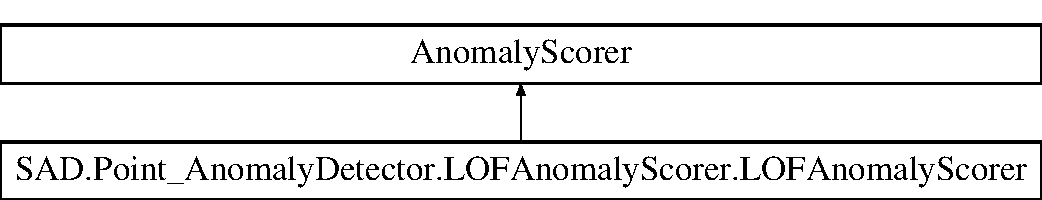
\includegraphics[height=2.000000cm]{classSAD_1_1Point__AnomalyDetector_1_1LOFAnomalyScorer_1_1LOFAnomalyScorer}
\end{center}
\end{figure}
\subsection*{Public Member Functions}
\begin{DoxyCompactItemize}
\item 
def \hyperlink{classSAD_1_1Point__AnomalyDetector_1_1LOFAnomalyScorer_1_1LOFAnomalyScorer_a901c20153f333b511bcfae6fb1c997a3}{\+\_\+\+\_\+init\+\_\+\+\_\+} (self, n\+\_\+neighbors=10, algorithm=\textquotesingle{}auto\textquotesingle{})
\item 
def \hyperlink{classSAD_1_1Point__AnomalyDetector_1_1LOFAnomalyScorer_1_1LOFAnomalyScorer_a1d4a77f8866cca6ed19db1f92ae13fd0}{Train\+\_\+\+Point\+Detector} (self, data)
\item 
def {\bfseries anomaly\+\_\+score} (self, data)\hypertarget{classSAD_1_1Point__AnomalyDetector_1_1LOFAnomalyScorer_1_1LOFAnomalyScorer_ad67e6c6a4abc10b5d9bfe54c066e94e4}{}\label{classSAD_1_1Point__AnomalyDetector_1_1LOFAnomalyScorer_1_1LOFAnomalyScorer_ad67e6c6a4abc10b5d9bfe54c066e94e4}

\item 
def {\bfseries fit\+\_\+incrementally} (self, data)\hypertarget{classSAD_1_1Point__AnomalyDetector_1_1LOFAnomalyScorer_1_1LOFAnomalyScorer_a09c724739e45504942bc135104077cc6}{}\label{classSAD_1_1Point__AnomalyDetector_1_1LOFAnomalyScorer_1_1LOFAnomalyScorer_a09c724739e45504942bc135104077cc6}

\end{DoxyCompactItemize}
\subsection*{Public Attributes}
\begin{DoxyCompactItemize}
\item 
{\bfseries n\+\_\+neighbors}\hypertarget{classSAD_1_1Point__AnomalyDetector_1_1LOFAnomalyScorer_1_1LOFAnomalyScorer_a25f6111d8c73e8e3dcac7009a27cf762}{}\label{classSAD_1_1Point__AnomalyDetector_1_1LOFAnomalyScorer_1_1LOFAnomalyScorer_a25f6111d8c73e8e3dcac7009a27cf762}

\item 
{\bfseries algorithm}\hypertarget{classSAD_1_1Point__AnomalyDetector_1_1LOFAnomalyScorer_1_1LOFAnomalyScorer_a60c856f4087c27a2048e1afe93f96193}{}\label{classSAD_1_1Point__AnomalyDetector_1_1LOFAnomalyScorer_1_1LOFAnomalyScorer_a60c856f4087c27a2048e1afe93f96193}

\item 
{\bfseries lof}\hypertarget{classSAD_1_1Point__AnomalyDetector_1_1LOFAnomalyScorer_1_1LOFAnomalyScorer_ac335b7ec6d13003eec655ba754c55921}{}\label{classSAD_1_1Point__AnomalyDetector_1_1LOFAnomalyScorer_1_1LOFAnomalyScorer_ac335b7ec6d13003eec655ba754c55921}

\end{DoxyCompactItemize}


\subsection{Constructor \& Destructor Documentation}
\index{S\+A\+D\+::\+Point\+\_\+\+Anomaly\+Detector\+::\+L\+O\+F\+Anomaly\+Scorer\+::\+L\+O\+F\+Anomaly\+Scorer@{S\+A\+D\+::\+Point\+\_\+\+Anomaly\+Detector\+::\+L\+O\+F\+Anomaly\+Scorer\+::\+L\+O\+F\+Anomaly\+Scorer}!\+\_\+\+\_\+init\+\_\+\+\_\+@{\+\_\+\+\_\+init\+\_\+\+\_\+}}
\index{\+\_\+\+\_\+init\+\_\+\+\_\+@{\+\_\+\+\_\+init\+\_\+\+\_\+}!S\+A\+D\+::\+Point\+\_\+\+Anomaly\+Detector\+::\+L\+O\+F\+Anomaly\+Scorer\+::\+L\+O\+F\+Anomaly\+Scorer@{S\+A\+D\+::\+Point\+\_\+\+Anomaly\+Detector\+::\+L\+O\+F\+Anomaly\+Scorer\+::\+L\+O\+F\+Anomaly\+Scorer}}
\subsubsection[{\texorpdfstring{\+\_\+\+\_\+init\+\_\+\+\_\+(self, n\+\_\+neighbors=10, algorithm=\textquotesingle{}auto\textquotesingle{})}{__init__(self, n_neighbors=10, algorithm='auto')}}]{\setlength{\rightskip}{0pt plus 5cm}def S\+A\+D.\+Point\+\_\+\+Anomaly\+Detector.\+L\+O\+F\+Anomaly\+Scorer.\+L\+O\+F\+Anomaly\+Scorer.\+\_\+\+\_\+init\+\_\+\+\_\+ (
\begin{DoxyParamCaption}
\item[{}]{self, }
\item[{}]{n\+\_\+neighbors = {\ttfamily 10}, }
\item[{}]{algorithm = {\ttfamily \textquotesingle{}auto\textquotesingle{}}}
\end{DoxyParamCaption}
)}\hypertarget{classSAD_1_1Point__AnomalyDetector_1_1LOFAnomalyScorer_1_1LOFAnomalyScorer_a901c20153f333b511bcfae6fb1c997a3}{}\label{classSAD_1_1Point__AnomalyDetector_1_1LOFAnomalyScorer_1_1LOFAnomalyScorer_a901c20153f333b511bcfae6fb1c997a3}
\begin{DoxyVerb}This is the point detector using lof algorithm
This by default needs the training phase
:param n_neighbors: number of the neighbors
:param algorithm: which algorithms to use, default auto
:return:
\end{DoxyVerb}
 

\subsection{Member Function Documentation}
\index{S\+A\+D\+::\+Point\+\_\+\+Anomaly\+Detector\+::\+L\+O\+F\+Anomaly\+Scorer\+::\+L\+O\+F\+Anomaly\+Scorer@{S\+A\+D\+::\+Point\+\_\+\+Anomaly\+Detector\+::\+L\+O\+F\+Anomaly\+Scorer\+::\+L\+O\+F\+Anomaly\+Scorer}!Train\+\_\+\+Point\+Detector@{Train\+\_\+\+Point\+Detector}}
\index{Train\+\_\+\+Point\+Detector@{Train\+\_\+\+Point\+Detector}!S\+A\+D\+::\+Point\+\_\+\+Anomaly\+Detector\+::\+L\+O\+F\+Anomaly\+Scorer\+::\+L\+O\+F\+Anomaly\+Scorer@{S\+A\+D\+::\+Point\+\_\+\+Anomaly\+Detector\+::\+L\+O\+F\+Anomaly\+Scorer\+::\+L\+O\+F\+Anomaly\+Scorer}}
\subsubsection[{\texorpdfstring{Train\+\_\+\+Point\+Detector(self, data)}{Train_PointDetector(self, data)}}]{\setlength{\rightskip}{0pt plus 5cm}def S\+A\+D.\+Point\+\_\+\+Anomaly\+Detector.\+L\+O\+F\+Anomaly\+Scorer.\+L\+O\+F\+Anomaly\+Scorer.\+Train\+\_\+\+Point\+Detector (
\begin{DoxyParamCaption}
\item[{}]{self, }
\item[{}]{data}
\end{DoxyParamCaption}
)}\hypertarget{classSAD_1_1Point__AnomalyDetector_1_1LOFAnomalyScorer_1_1LOFAnomalyScorer_a1d4a77f8866cca6ed19db1f92ae13fd0}{}\label{classSAD_1_1Point__AnomalyDetector_1_1LOFAnomalyScorer_1_1LOFAnomalyScorer_a1d4a77f8866cca6ed19db1f92ae13fd0}
\begin{DoxyVerb}For training the point detector
:param data: the input for training the point detector
:return:
\end{DoxyVerb}
 

The documentation for this class was generated from the following file\+:\begin{DoxyCompactItemize}
\item 
Point\+\_\+\+Anomaly\+Detector/L\+O\+F\+Anomaly\+Scorer.\+py\end{DoxyCompactItemize}

\input{classSAD_1_1Stream__AnomalyDetector_1_1PRAAG_1_1PRAAG}
\hypertarget{classSAD_1_1Point__AnomalyDetector_1_1PyiscAnomalyScorer_1_1PyiscAnomalyScorer}{}\section{S\+A\+D.\+Point\+\_\+\+Anomaly\+Detector.\+Pyisc\+Anomaly\+Scorer.\+Pyisc\+Anomaly\+Scorer Class Reference}
\label{classSAD_1_1Point__AnomalyDetector_1_1PyiscAnomalyScorer_1_1PyiscAnomalyScorer}\index{S\+A\+D.\+Point\+\_\+\+Anomaly\+Detector.\+Pyisc\+Anomaly\+Scorer.\+Pyisc\+Anomaly\+Scorer@{S\+A\+D.\+Point\+\_\+\+Anomaly\+Detector.\+Pyisc\+Anomaly\+Scorer.\+Pyisc\+Anomaly\+Scorer}}
Inheritance diagram for S\+A\+D.\+Point\+\_\+\+Anomaly\+Detector.\+Pyisc\+Anomaly\+Scorer.\+Pyisc\+Anomaly\+Scorer\+:\begin{figure}[H]
\begin{center}
\leavevmode
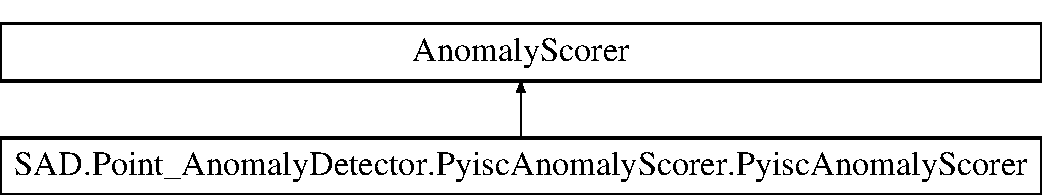
\includegraphics[height=2.000000cm]{classSAD_1_1Point__AnomalyDetector_1_1PyiscAnomalyScorer_1_1PyiscAnomalyScorer}
\end{center}
\end{figure}
\subsection*{Public Member Functions}
\begin{DoxyCompactItemize}
\item 
def \hyperlink{classSAD_1_1Point__AnomalyDetector_1_1PyiscAnomalyScorer_1_1PyiscAnomalyScorer_abc3bc5cec9cb7a036e27d38fd754a971}{\+\_\+\+\_\+init\+\_\+\+\_\+} (self, models=\mbox{[}$\,$\mbox{]})
\item 
def \hyperlink{classSAD_1_1Point__AnomalyDetector_1_1PyiscAnomalyScorer_1_1PyiscAnomalyScorer_ae27cbcb8c835a0fa016b9eafa4045052}{Train\+\_\+\+Point\+Detector} (self, data=\mbox{[}$\,$\mbox{]})
\end{DoxyCompactItemize}
\subsection*{Public Attributes}
\begin{DoxyCompactItemize}
\item 
{\bfseries Fit\+\_\+data}\hypertarget{classSAD_1_1Point__AnomalyDetector_1_1PyiscAnomalyScorer_1_1PyiscAnomalyScorer_a48edccc0d69161cf1e0787ea9597d9d6}{}\label{classSAD_1_1Point__AnomalyDetector_1_1PyiscAnomalyScorer_1_1PyiscAnomalyScorer_a48edccc0d69161cf1e0787ea9597d9d6}

\item 
{\bfseries component\+\_\+models}\hypertarget{classSAD_1_1Point__AnomalyDetector_1_1PyiscAnomalyScorer_1_1PyiscAnomalyScorer_ab0acbf34c58d6323750d493b75b85e6f}{}\label{classSAD_1_1Point__AnomalyDetector_1_1PyiscAnomalyScorer_1_1PyiscAnomalyScorer_ab0acbf34c58d6323750d493b75b85e6f}

\end{DoxyCompactItemize}


\subsection{Constructor \& Destructor Documentation}
\index{S\+A\+D\+::\+Point\+\_\+\+Anomaly\+Detector\+::\+Pyisc\+Anomaly\+Scorer\+::\+Pyisc\+Anomaly\+Scorer@{S\+A\+D\+::\+Point\+\_\+\+Anomaly\+Detector\+::\+Pyisc\+Anomaly\+Scorer\+::\+Pyisc\+Anomaly\+Scorer}!\+\_\+\+\_\+init\+\_\+\+\_\+@{\+\_\+\+\_\+init\+\_\+\+\_\+}}
\index{\+\_\+\+\_\+init\+\_\+\+\_\+@{\+\_\+\+\_\+init\+\_\+\+\_\+}!S\+A\+D\+::\+Point\+\_\+\+Anomaly\+Detector\+::\+Pyisc\+Anomaly\+Scorer\+::\+Pyisc\+Anomaly\+Scorer@{S\+A\+D\+::\+Point\+\_\+\+Anomaly\+Detector\+::\+Pyisc\+Anomaly\+Scorer\+::\+Pyisc\+Anomaly\+Scorer}}
\subsubsection[{\texorpdfstring{\+\_\+\+\_\+init\+\_\+\+\_\+(self, models=[])}{__init__(self, models=[])}}]{\setlength{\rightskip}{0pt plus 5cm}def S\+A\+D.\+Point\+\_\+\+Anomaly\+Detector.\+Pyisc\+Anomaly\+Scorer.\+Pyisc\+Anomaly\+Scorer.\+\_\+\+\_\+init\+\_\+\+\_\+ (
\begin{DoxyParamCaption}
\item[{}]{self, }
\item[{}]{models = {\ttfamily \mbox{[}\mbox{]}}}
\end{DoxyParamCaption}
)}\hypertarget{classSAD_1_1Point__AnomalyDetector_1_1PyiscAnomalyScorer_1_1PyiscAnomalyScorer_abc3bc5cec9cb7a036e27d38fd754a971}{}\label{classSAD_1_1Point__AnomalyDetector_1_1PyiscAnomalyScorer_1_1PyiscAnomalyScorer_abc3bc5cec9cb7a036e27d38fd754a971}
\begin{DoxyVerb}This is the point detector using pyisc framework
There is no training phase for this framework, all the distributions are in models
:param models: input the component models for pyisc, useful for the incremental implementation
:return:
\end{DoxyVerb}
 

\subsection{Member Function Documentation}
\index{S\+A\+D\+::\+Point\+\_\+\+Anomaly\+Detector\+::\+Pyisc\+Anomaly\+Scorer\+::\+Pyisc\+Anomaly\+Scorer@{S\+A\+D\+::\+Point\+\_\+\+Anomaly\+Detector\+::\+Pyisc\+Anomaly\+Scorer\+::\+Pyisc\+Anomaly\+Scorer}!Train\+\_\+\+Point\+Detector@{Train\+\_\+\+Point\+Detector}}
\index{Train\+\_\+\+Point\+Detector@{Train\+\_\+\+Point\+Detector}!S\+A\+D\+::\+Point\+\_\+\+Anomaly\+Detector\+::\+Pyisc\+Anomaly\+Scorer\+::\+Pyisc\+Anomaly\+Scorer@{S\+A\+D\+::\+Point\+\_\+\+Anomaly\+Detector\+::\+Pyisc\+Anomaly\+Scorer\+::\+Pyisc\+Anomaly\+Scorer}}
\subsubsection[{\texorpdfstring{Train\+\_\+\+Point\+Detector(self, data=[])}{Train_PointDetector(self, data=[])}}]{\setlength{\rightskip}{0pt plus 5cm}def S\+A\+D.\+Point\+\_\+\+Anomaly\+Detector.\+Pyisc\+Anomaly\+Scorer.\+Pyisc\+Anomaly\+Scorer.\+Train\+\_\+\+Point\+Detector (
\begin{DoxyParamCaption}
\item[{}]{self, }
\item[{}]{data = {\ttfamily \mbox{[}\mbox{]}}}
\end{DoxyParamCaption}
)}\hypertarget{classSAD_1_1Point__AnomalyDetector_1_1PyiscAnomalyScorer_1_1PyiscAnomalyScorer_ae27cbcb8c835a0fa016b9eafa4045052}{}\label{classSAD_1_1Point__AnomalyDetector_1_1PyiscAnomalyScorer_1_1PyiscAnomalyScorer_ae27cbcb8c835a0fa016b9eafa4045052}
\begin{DoxyVerb}:param data: train the point detector according to the data
:return:
\end{DoxyVerb}
 

The documentation for this class was generated from the following file\+:\begin{DoxyCompactItemize}
\item 
Point\+\_\+\+Anomaly\+Detector/Pyisc\+Anomaly\+Scorer.\+py\end{DoxyCompactItemize}

\hypertarget{classSAD_1_1Point__AnomalyDetector_1_1PyiscAnomalyScorer__advanced_1_1PyiscAnomalyScorer__advanced}{}\section{S\+A\+D.\+Point\+\_\+\+Anomaly\+Detector.\+Pyisc\+Anomaly\+Scorer\+\_\+advanced.\+Pyisc\+Anomaly\+Scorer\+\_\+advanced Class Reference}
\label{classSAD_1_1Point__AnomalyDetector_1_1PyiscAnomalyScorer__advanced_1_1PyiscAnomalyScorer__advanced}\index{S\+A\+D.\+Point\+\_\+\+Anomaly\+Detector.\+Pyisc\+Anomaly\+Scorer\+\_\+advanced.\+Pyisc\+Anomaly\+Scorer\+\_\+advanced@{S\+A\+D.\+Point\+\_\+\+Anomaly\+Detector.\+Pyisc\+Anomaly\+Scorer\+\_\+advanced.\+Pyisc\+Anomaly\+Scorer\+\_\+advanced}}
Inheritance diagram for S\+A\+D.\+Point\+\_\+\+Anomaly\+Detector.\+Pyisc\+Anomaly\+Scorer\+\_\+advanced.\+Pyisc\+Anomaly\+Scorer\+\_\+advanced\+:\begin{figure}[H]
\begin{center}
\leavevmode
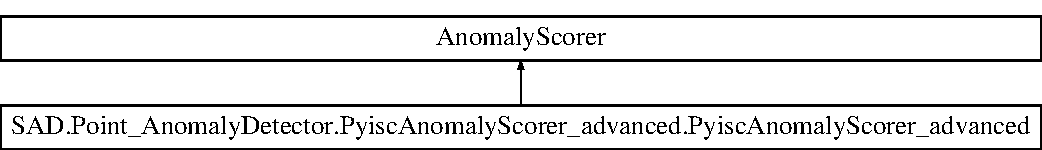
\includegraphics[height=2.000000cm]{classSAD_1_1Point__AnomalyDetector_1_1PyiscAnomalyScorer__advanced_1_1PyiscAnomalyScorer__advanced}
\end{center}
\end{figure}
\subsection*{Public Member Functions}
\begin{DoxyCompactItemize}
\item 
def \hyperlink{classSAD_1_1Point__AnomalyDetector_1_1PyiscAnomalyScorer__advanced_1_1PyiscAnomalyScorer__advanced_a0f31a799a55ffef102c814a436661d10}{\+\_\+\+\_\+init\+\_\+\+\_\+} (self, dist=\mbox{[}\textquotesingle{}norm\textquotesingle{}\mbox{]})
\item 
def \hyperlink{classSAD_1_1Point__AnomalyDetector_1_1PyiscAnomalyScorer__advanced_1_1PyiscAnomalyScorer__advanced_aef70b902dc9c5df150eecd5c0b1c3916}{Train\+\_\+\+Point\+Detector} (self, data)
\end{DoxyCompactItemize}
\subsection*{Public Attributes}
\begin{DoxyCompactItemize}
\item 
{\bfseries Fit\+\_\+data}\hypertarget{classSAD_1_1Point__AnomalyDetector_1_1PyiscAnomalyScorer__advanced_1_1PyiscAnomalyScorer__advanced_a562d1e9828fbdc6a95436452dddbc3b8}{}\label{classSAD_1_1Point__AnomalyDetector_1_1PyiscAnomalyScorer__advanced_1_1PyiscAnomalyScorer__advanced_a562d1e9828fbdc6a95436452dddbc3b8}

\item 
{\bfseries test\+\_\+distribution}\hypertarget{classSAD_1_1Point__AnomalyDetector_1_1PyiscAnomalyScorer__advanced_1_1PyiscAnomalyScorer__advanced_aaefabc087f5917aa7426745c93e4f5cb}{}\label{classSAD_1_1Point__AnomalyDetector_1_1PyiscAnomalyScorer__advanced_1_1PyiscAnomalyScorer__advanced_aaefabc087f5917aa7426745c93e4f5cb}

\end{DoxyCompactItemize}


\subsection{Constructor \& Destructor Documentation}
\index{S\+A\+D\+::\+Point\+\_\+\+Anomaly\+Detector\+::\+Pyisc\+Anomaly\+Scorer\+\_\+advanced\+::\+Pyisc\+Anomaly\+Scorer\+\_\+advanced@{S\+A\+D\+::\+Point\+\_\+\+Anomaly\+Detector\+::\+Pyisc\+Anomaly\+Scorer\+\_\+advanced\+::\+Pyisc\+Anomaly\+Scorer\+\_\+advanced}!\+\_\+\+\_\+init\+\_\+\+\_\+@{\+\_\+\+\_\+init\+\_\+\+\_\+}}
\index{\+\_\+\+\_\+init\+\_\+\+\_\+@{\+\_\+\+\_\+init\+\_\+\+\_\+}!S\+A\+D\+::\+Point\+\_\+\+Anomaly\+Detector\+::\+Pyisc\+Anomaly\+Scorer\+\_\+advanced\+::\+Pyisc\+Anomaly\+Scorer\+\_\+advanced@{S\+A\+D\+::\+Point\+\_\+\+Anomaly\+Detector\+::\+Pyisc\+Anomaly\+Scorer\+\_\+advanced\+::\+Pyisc\+Anomaly\+Scorer\+\_\+advanced}}
\subsubsection[{\texorpdfstring{\+\_\+\+\_\+init\+\_\+\+\_\+(self, dist=[\textquotesingle{}norm\textquotesingle{}])}{__init__(self, dist=['norm'])}}]{\setlength{\rightskip}{0pt plus 5cm}def S\+A\+D.\+Point\+\_\+\+Anomaly\+Detector.\+Pyisc\+Anomaly\+Scorer\+\_\+advanced.\+Pyisc\+Anomaly\+Scorer\+\_\+advanced.\+\_\+\+\_\+init\+\_\+\+\_\+ (
\begin{DoxyParamCaption}
\item[{}]{self, }
\item[{}]{dist = {\ttfamily \mbox{[}\textquotesingle{}norm\textquotesingle{}\mbox{]}}}
\end{DoxyParamCaption}
)}\hypertarget{classSAD_1_1Point__AnomalyDetector_1_1PyiscAnomalyScorer__advanced_1_1PyiscAnomalyScorer__advanced_a0f31a799a55ffef102c814a436661d10}{}\label{classSAD_1_1Point__AnomalyDetector_1_1PyiscAnomalyScorer__advanced_1_1PyiscAnomalyScorer__advanced_a0f31a799a55ffef102c814a436661d10}
\begin{DoxyVerb}This is the point detector from pyisc framework
There is training phase which will fit the data in distributions in dist and also poisson
:param dist: the distributions for pyisc which wants to be tried, see distributions in Fit_data
:return:
\end{DoxyVerb}
 

\subsection{Member Function Documentation}
\index{S\+A\+D\+::\+Point\+\_\+\+Anomaly\+Detector\+::\+Pyisc\+Anomaly\+Scorer\+\_\+advanced\+::\+Pyisc\+Anomaly\+Scorer\+\_\+advanced@{S\+A\+D\+::\+Point\+\_\+\+Anomaly\+Detector\+::\+Pyisc\+Anomaly\+Scorer\+\_\+advanced\+::\+Pyisc\+Anomaly\+Scorer\+\_\+advanced}!Train\+\_\+\+Point\+Detector@{Train\+\_\+\+Point\+Detector}}
\index{Train\+\_\+\+Point\+Detector@{Train\+\_\+\+Point\+Detector}!S\+A\+D\+::\+Point\+\_\+\+Anomaly\+Detector\+::\+Pyisc\+Anomaly\+Scorer\+\_\+advanced\+::\+Pyisc\+Anomaly\+Scorer\+\_\+advanced@{S\+A\+D\+::\+Point\+\_\+\+Anomaly\+Detector\+::\+Pyisc\+Anomaly\+Scorer\+\_\+advanced\+::\+Pyisc\+Anomaly\+Scorer\+\_\+advanced}}
\subsubsection[{\texorpdfstring{Train\+\_\+\+Point\+Detector(self, data)}{Train_PointDetector(self, data)}}]{\setlength{\rightskip}{0pt plus 5cm}def S\+A\+D.\+Point\+\_\+\+Anomaly\+Detector.\+Pyisc\+Anomaly\+Scorer\+\_\+advanced.\+Pyisc\+Anomaly\+Scorer\+\_\+advanced.\+Train\+\_\+\+Point\+Detector (
\begin{DoxyParamCaption}
\item[{}]{self, }
\item[{}]{data}
\end{DoxyParamCaption}
)}\hypertarget{classSAD_1_1Point__AnomalyDetector_1_1PyiscAnomalyScorer__advanced_1_1PyiscAnomalyScorer__advanced_aef70b902dc9c5df150eecd5c0b1c3916}{}\label{classSAD_1_1Point__AnomalyDetector_1_1PyiscAnomalyScorer__advanced_1_1PyiscAnomalyScorer__advanced_aef70b902dc9c5df150eecd5c0b1c3916}
\begin{DoxyVerb}:param data: The data which is used for training
:return:
\end{DoxyVerb}
 

The documentation for this class was generated from the following file\+:\begin{DoxyCompactItemize}
\item 
Point\+\_\+\+Anomaly\+Detector/Pyisc\+Anomaly\+Scorer\+\_\+advanced.\+py\end{DoxyCompactItemize}

\hypertarget{classSAD_1_1Stream__Generator_1_1Simulation__Generator_1_1Simulation__Generator}{}\section{S\+A\+D.\+Stream\+\_\+\+Generator.\+Simulation\+\_\+\+Generator.\+Simulation\+\_\+\+Generator Class Reference}
\label{classSAD_1_1Stream__Generator_1_1Simulation__Generator_1_1Simulation__Generator}\index{S\+A\+D.\+Stream\+\_\+\+Generator.\+Simulation\+\_\+\+Generator.\+Simulation\+\_\+\+Generator@{S\+A\+D.\+Stream\+\_\+\+Generator.\+Simulation\+\_\+\+Generator.\+Simulation\+\_\+\+Generator}}


Inheritance diagram for S\+A\+D.\+Stream\+\_\+\+Generator.\+Simulation\+\_\+\+Generator.\+Simulation\+\_\+\+Generator\+:\nopagebreak
\begin{figure}[H]
\begin{center}
\leavevmode
\includegraphics[width=248pt]{classSAD_1_1Stream__Generator_1_1Simulation__Generator_1_1Simulation__Generator__inherit__graph}
\end{center}
\end{figure}


Collaboration diagram for S\+A\+D.\+Stream\+\_\+\+Generator.\+Simulation\+\_\+\+Generator.\+Simulation\+\_\+\+Generator\+:\nopagebreak
\begin{figure}[H]
\begin{center}
\leavevmode
\includegraphics[width=248pt]{classSAD_1_1Stream__Generator_1_1Simulation__Generator_1_1Simulation__Generator__coll__graph}
\end{center}
\end{figure}
\subsection*{Public Member Functions}
\begin{DoxyCompactItemize}
\item 
def \hyperlink{classSAD_1_1Stream__Generator_1_1Simulation__Generator_1_1Simulation__Generator_a2103b42b5bcb5cf441e74de526695f86}{\+\_\+\+\_\+init\+\_\+\+\_\+} (self, list\+\_\+distribution, normal\+\_\+error\+\_\+distribution, anomaly\+\_\+error\+\_\+distribution, type\+\_\+error=\char`\"{}Sudden\char`\"{})
\item 
def \hyperlink{classSAD_1_1Stream__Generator_1_1Simulation__Generator_1_1Simulation__Generator_a0ca784a29449c50c31db5a171ea3c378}{Generate\+\_\+\+Train\+Data} (self, number)
\item 
def \hyperlink{classSAD_1_1Stream__Generator_1_1Simulation__Generator_1_1Simulation__Generator_ab3812dceb7cec4fdac22dae14f72b793}{Generate\+\_\+\+Stream} (self, type, number)
\end{DoxyCompactItemize}
\subsection*{Public Attributes}
\begin{DoxyCompactItemize}
\item 
{\bfseries list\+\_\+distribution}\hypertarget{classSAD_1_1Stream__Generator_1_1Simulation__Generator_1_1Simulation__Generator_ada97d143aed23d023a14802be273cc43}{}\label{classSAD_1_1Stream__Generator_1_1Simulation__Generator_1_1Simulation__Generator_ada97d143aed23d023a14802be273cc43}

\item 
{\bfseries normal\+\_\+error\+\_\+distribution}\hypertarget{classSAD_1_1Stream__Generator_1_1Simulation__Generator_1_1Simulation__Generator_ac82d794c9ff18c9ed18b37d99acbd310}{}\label{classSAD_1_1Stream__Generator_1_1Simulation__Generator_1_1Simulation__Generator_ac82d794c9ff18c9ed18b37d99acbd310}

\item 
{\bfseries anomaly\+\_\+error\+\_\+distribution}\hypertarget{classSAD_1_1Stream__Generator_1_1Simulation__Generator_1_1Simulation__Generator_a3b5f692bcddf70d6f0aa71c4368a1ed9}{}\label{classSAD_1_1Stream__Generator_1_1Simulation__Generator_1_1Simulation__Generator_a3b5f692bcddf70d6f0aa71c4368a1ed9}

\item 
{\bfseries type\+\_\+error}\hypertarget{classSAD_1_1Stream__Generator_1_1Simulation__Generator_1_1Simulation__Generator_a25fe829176c8ace01af7fb47f4a622b2}{}\label{classSAD_1_1Stream__Generator_1_1Simulation__Generator_1_1Simulation__Generator_a25fe829176c8ace01af7fb47f4a622b2}

\end{DoxyCompactItemize}


\subsection{Constructor \& Destructor Documentation}
\index{S\+A\+D\+::\+Stream\+\_\+\+Generator\+::\+Simulation\+\_\+\+Generator\+::\+Simulation\+\_\+\+Generator@{S\+A\+D\+::\+Stream\+\_\+\+Generator\+::\+Simulation\+\_\+\+Generator\+::\+Simulation\+\_\+\+Generator}!\+\_\+\+\_\+init\+\_\+\+\_\+@{\+\_\+\+\_\+init\+\_\+\+\_\+}}
\index{\+\_\+\+\_\+init\+\_\+\+\_\+@{\+\_\+\+\_\+init\+\_\+\+\_\+}!S\+A\+D\+::\+Stream\+\_\+\+Generator\+::\+Simulation\+\_\+\+Generator\+::\+Simulation\+\_\+\+Generator@{S\+A\+D\+::\+Stream\+\_\+\+Generator\+::\+Simulation\+\_\+\+Generator\+::\+Simulation\+\_\+\+Generator}}
\subsubsection[{\texorpdfstring{\+\_\+\+\_\+init\+\_\+\+\_\+(self, list\+\_\+distribution, normal\+\_\+error\+\_\+distribution, anomaly\+\_\+error\+\_\+distribution, type\+\_\+error=""Sudden"")}{__init__(self, list_distribution, normal_error_distribution, anomaly_error_distribution, type_error="Sudden")}}]{\setlength{\rightskip}{0pt plus 5cm}def S\+A\+D.\+Stream\+\_\+\+Generator.\+Simulation\+\_\+\+Generator.\+Simulation\+\_\+\+Generator.\+\_\+\+\_\+init\+\_\+\+\_\+ (
\begin{DoxyParamCaption}
\item[{}]{self, }
\item[{}]{list\+\_\+distribution, }
\item[{}]{normal\+\_\+error\+\_\+distribution, }
\item[{}]{anomaly\+\_\+error\+\_\+distribution, }
\item[{}]{type\+\_\+error = {\ttfamily \char`\"{}Sudden\char`\"{}}}
\end{DoxyParamCaption}
)}\hypertarget{classSAD_1_1Stream__Generator_1_1Simulation__Generator_1_1Simulation__Generator_a2103b42b5bcb5cf441e74de526695f86}{}\label{classSAD_1_1Stream__Generator_1_1Simulation__Generator_1_1Simulation__Generator_a2103b42b5bcb5cf441e74de526695f86}
\begin{DoxyVerb}For generating the siulation stream data, the features are in list_distributions
If the need training phase, also used for generating train_data
For stream data, they could generate errors from type_error
:param list_distribution: the distribution type for normal cases
:param normal_error_distribution:the error distribution types for normal cases
:param anomaly_error_distribution:the error distribution types for anomaly cases
:param type_error: the error type for the stream
:return:
\end{DoxyVerb}
 

\subsection{Member Function Documentation}
\index{S\+A\+D\+::\+Stream\+\_\+\+Generator\+::\+Simulation\+\_\+\+Generator\+::\+Simulation\+\_\+\+Generator@{S\+A\+D\+::\+Stream\+\_\+\+Generator\+::\+Simulation\+\_\+\+Generator\+::\+Simulation\+\_\+\+Generator}!Generate\+\_\+\+Stream@{Generate\+\_\+\+Stream}}
\index{Generate\+\_\+\+Stream@{Generate\+\_\+\+Stream}!S\+A\+D\+::\+Stream\+\_\+\+Generator\+::\+Simulation\+\_\+\+Generator\+::\+Simulation\+\_\+\+Generator@{S\+A\+D\+::\+Stream\+\_\+\+Generator\+::\+Simulation\+\_\+\+Generator\+::\+Simulation\+\_\+\+Generator}}
\subsubsection[{\texorpdfstring{Generate\+\_\+\+Stream(self, type, number)}{Generate_Stream(self, type, number)}}]{\setlength{\rightskip}{0pt plus 5cm}def S\+A\+D.\+Stream\+\_\+\+Generator.\+Simulation\+\_\+\+Generator.\+Simulation\+\_\+\+Generator.\+Generate\+\_\+\+Stream (
\begin{DoxyParamCaption}
\item[{}]{self, }
\item[{}]{type, }
\item[{}]{number}
\end{DoxyParamCaption}
)}\hypertarget{classSAD_1_1Stream__Generator_1_1Simulation__Generator_1_1Simulation__Generator_ab3812dceb7cec4fdac22dae14f72b793}{}\label{classSAD_1_1Stream__Generator_1_1Simulation__Generator_1_1Simulation__Generator_ab3812dceb7cec4fdac22dae14f72b793}
\begin{DoxyVerb}:param type: type is either normal or anomaly
:param number: number of the stream data generated
:return: the matrix of the stream data according to the distribution and type
\end{DoxyVerb}
 \index{S\+A\+D\+::\+Stream\+\_\+\+Generator\+::\+Simulation\+\_\+\+Generator\+::\+Simulation\+\_\+\+Generator@{S\+A\+D\+::\+Stream\+\_\+\+Generator\+::\+Simulation\+\_\+\+Generator\+::\+Simulation\+\_\+\+Generator}!Generate\+\_\+\+Train\+Data@{Generate\+\_\+\+Train\+Data}}
\index{Generate\+\_\+\+Train\+Data@{Generate\+\_\+\+Train\+Data}!S\+A\+D\+::\+Stream\+\_\+\+Generator\+::\+Simulation\+\_\+\+Generator\+::\+Simulation\+\_\+\+Generator@{S\+A\+D\+::\+Stream\+\_\+\+Generator\+::\+Simulation\+\_\+\+Generator\+::\+Simulation\+\_\+\+Generator}}
\subsubsection[{\texorpdfstring{Generate\+\_\+\+Train\+Data(self, number)}{Generate_TrainData(self, number)}}]{\setlength{\rightskip}{0pt plus 5cm}def S\+A\+D.\+Stream\+\_\+\+Generator.\+Simulation\+\_\+\+Generator.\+Simulation\+\_\+\+Generator.\+Generate\+\_\+\+Train\+Data (
\begin{DoxyParamCaption}
\item[{}]{self, }
\item[{}]{number}
\end{DoxyParamCaption}
)}\hypertarget{classSAD_1_1Stream__Generator_1_1Simulation__Generator_1_1Simulation__Generator_a0ca784a29449c50c31db5a171ea3c378}{}\label{classSAD_1_1Stream__Generator_1_1Simulation__Generator_1_1Simulation__Generator_a0ca784a29449c50c31db5a171ea3c378}
\begin{DoxyVerb}:param number: number of the data generated for training
:return: the matrix of the training data according to the distribution
\end{DoxyVerb}
 

The documentation for this class was generated from the following file\+:\begin{DoxyCompactItemize}
\item 
Stream\+\_\+\+Generator/Simulation\+\_\+\+Generator.\+py\end{DoxyCompactItemize}

\hypertarget{classSAD_1_1Stream__AnomalyDetector_1_1Stream__Detector_1_1Stream__Detector}{}\section{S\+A\+D.\+Stream\+\_\+\+Anomaly\+Detector.\+Stream\+\_\+\+Detector.\+Stream\+\_\+\+Detector Class Reference}
\label{classSAD_1_1Stream__AnomalyDetector_1_1Stream__Detector_1_1Stream__Detector}\index{S\+A\+D.\+Stream\+\_\+\+Anomaly\+Detector.\+Stream\+\_\+\+Detector.\+Stream\+\_\+\+Detector@{S\+A\+D.\+Stream\+\_\+\+Anomaly\+Detector.\+Stream\+\_\+\+Detector.\+Stream\+\_\+\+Detector}}


Inheritance diagram for S\+A\+D.\+Stream\+\_\+\+Anomaly\+Detector.\+Stream\+\_\+\+Detector.\+Stream\+\_\+\+Detector\+:\nopagebreak
\begin{figure}[H]
\begin{center}
\leavevmode
\includegraphics[width=246pt]{classSAD_1_1Stream__AnomalyDetector_1_1Stream__Detector_1_1Stream__Detector__inherit__graph}
\end{center}
\end{figure}


Collaboration diagram for S\+A\+D.\+Stream\+\_\+\+Anomaly\+Detector.\+Stream\+\_\+\+Detector.\+Stream\+\_\+\+Detector\+:\nopagebreak
\begin{figure}[H]
\begin{center}
\leavevmode
\includegraphics[width=246pt]{classSAD_1_1Stream__AnomalyDetector_1_1Stream__Detector_1_1Stream__Detector__coll__graph}
\end{center}
\end{figure}
\subsection*{Public Member Functions}
\begin{DoxyCompactItemize}
\item 
def \hyperlink{classSAD_1_1Stream__AnomalyDetector_1_1Stream__Detector_1_1Stream__Detector_ab0755de610c22dfb6b2bbdfce4ec5d67}{\+\_\+\+\_\+init\+\_\+\+\_\+} (self, para=0.\+0)
\item 
def \hyperlink{classSAD_1_1Stream__AnomalyDetector_1_1Stream__Detector_1_1Stream__Detector_ab1cad60e8f3996d3cf8aae56111f356b}{check} (self, score=0.\+0)
\end{DoxyCompactItemize}


\subsection{Constructor \& Destructor Documentation}
\index{S\+A\+D\+::\+Stream\+\_\+\+Anomaly\+Detector\+::\+Stream\+\_\+\+Detector\+::\+Stream\+\_\+\+Detector@{S\+A\+D\+::\+Stream\+\_\+\+Anomaly\+Detector\+::\+Stream\+\_\+\+Detector\+::\+Stream\+\_\+\+Detector}!\+\_\+\+\_\+init\+\_\+\+\_\+@{\+\_\+\+\_\+init\+\_\+\+\_\+}}
\index{\+\_\+\+\_\+init\+\_\+\+\_\+@{\+\_\+\+\_\+init\+\_\+\+\_\+}!S\+A\+D\+::\+Stream\+\_\+\+Anomaly\+Detector\+::\+Stream\+\_\+\+Detector\+::\+Stream\+\_\+\+Detector@{S\+A\+D\+::\+Stream\+\_\+\+Anomaly\+Detector\+::\+Stream\+\_\+\+Detector\+::\+Stream\+\_\+\+Detector}}
\subsubsection[{\texorpdfstring{\+\_\+\+\_\+init\+\_\+\+\_\+(self, para=0.\+0)}{__init__(self, para=0.0)}}]{\setlength{\rightskip}{0pt plus 5cm}def S\+A\+D.\+Stream\+\_\+\+Anomaly\+Detector.\+Stream\+\_\+\+Detector.\+Stream\+\_\+\+Detector.\+\_\+\+\_\+init\+\_\+\+\_\+ (
\begin{DoxyParamCaption}
\item[{}]{self, }
\item[{}]{para = {\ttfamily 0.0}}
\end{DoxyParamCaption}
)}\hypertarget{classSAD_1_1Stream__AnomalyDetector_1_1Stream__Detector_1_1Stream__Detector_ab0755de610c22dfb6b2bbdfce4ec5d67}{}\label{classSAD_1_1Stream__AnomalyDetector_1_1Stream__Detector_1_1Stream__Detector_ab0755de610c22dfb6b2bbdfce4ec5d67}
\begin{DoxyVerb}This is the super class for Stream_detector
:param para:
:return:
\end{DoxyVerb}
 

\subsection{Member Function Documentation}
\index{S\+A\+D\+::\+Stream\+\_\+\+Anomaly\+Detector\+::\+Stream\+\_\+\+Detector\+::\+Stream\+\_\+\+Detector@{S\+A\+D\+::\+Stream\+\_\+\+Anomaly\+Detector\+::\+Stream\+\_\+\+Detector\+::\+Stream\+\_\+\+Detector}!check@{check}}
\index{check@{check}!S\+A\+D\+::\+Stream\+\_\+\+Anomaly\+Detector\+::\+Stream\+\_\+\+Detector\+::\+Stream\+\_\+\+Detector@{S\+A\+D\+::\+Stream\+\_\+\+Anomaly\+Detector\+::\+Stream\+\_\+\+Detector\+::\+Stream\+\_\+\+Detector}}
\subsubsection[{\texorpdfstring{check(self, score=0.\+0)}{check(self, score=0.0)}}]{\setlength{\rightskip}{0pt plus 5cm}def S\+A\+D.\+Stream\+\_\+\+Anomaly\+Detector.\+Stream\+\_\+\+Detector.\+Stream\+\_\+\+Detector.\+check (
\begin{DoxyParamCaption}
\item[{}]{self, }
\item[{}]{score = {\ttfamily 0.0}}
\end{DoxyParamCaption}
)}\hypertarget{classSAD_1_1Stream__AnomalyDetector_1_1Stream__Detector_1_1Stream__Detector_ab1cad60e8f3996d3cf8aae56111f356b}{}\label{classSAD_1_1Stream__AnomalyDetector_1_1Stream__Detector_1_1Stream__Detector_ab1cad60e8f3996d3cf8aae56111f356b}
\begin{DoxyVerb}This is for checking whether there is anomalous happening when a new score comes
:param score: The score from the point detector
:return:
\end{DoxyVerb}
 

The documentation for this class was generated from the following file\+:\begin{DoxyCompactItemize}
\item 
Stream\+\_\+\+Anomaly\+Detector/Stream\+\_\+\+Detector.\+py\end{DoxyCompactItemize}

\input{classSAD_1_1Point__AnomalyDetector_1_1SVMAnomalyScorer_1_1SVMAnomalyScorer}
\hypertarget{classSAD_1_1Stream__Generator_1_1Timestamp__Dataset__Generator_1_1Timestamp__Dataset__Generator}{}\section{S\+A\+D.\+Stream\+\_\+\+Generator.\+Timestamp\+\_\+\+Dataset\+\_\+\+Generator.\+Timestamp\+\_\+\+Dataset\+\_\+\+Generator Class Reference}
\label{classSAD_1_1Stream__Generator_1_1Timestamp__Dataset__Generator_1_1Timestamp__Dataset__Generator}\index{S\+A\+D.\+Stream\+\_\+\+Generator.\+Timestamp\+\_\+\+Dataset\+\_\+\+Generator.\+Timestamp\+\_\+\+Dataset\+\_\+\+Generator@{S\+A\+D.\+Stream\+\_\+\+Generator.\+Timestamp\+\_\+\+Dataset\+\_\+\+Generator.\+Timestamp\+\_\+\+Dataset\+\_\+\+Generator}}
Inheritance diagram for S\+A\+D.\+Stream\+\_\+\+Generator.\+Timestamp\+\_\+\+Dataset\+\_\+\+Generator.\+Timestamp\+\_\+\+Dataset\+\_\+\+Generator\+:\begin{figure}[H]
\begin{center}
\leavevmode
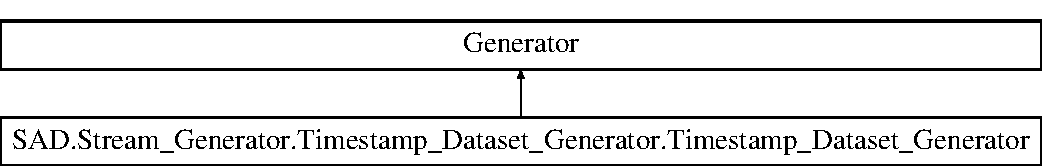
\includegraphics[height=2.000000cm]{classSAD_1_1Stream__Generator_1_1Timestamp__Dataset__Generator_1_1Timestamp__Dataset__Generator}
\end{center}
\end{figure}
\subsection*{Public Member Functions}
\begin{DoxyCompactItemize}
\item 
def \hyperlink{classSAD_1_1Stream__Generator_1_1Timestamp__Dataset__Generator_1_1Timestamp__Dataset__Generator_a5c48488d2bc6122cddc3f0c68587b820}{\+\_\+\+\_\+init\+\_\+\+\_\+} (self, filename, delimiter=\char`\"{},  del\+\_\+timestamp\+\_\+column=True,  timestamp\+\_\+column=0)
\item 
def \hyperlink{classSAD_1_1Stream__Generator_1_1Timestamp__Dataset__Generator_1_1Timestamp__Dataset__Generator_a90679f7d1b4dab5dbff87b7f44cba086}{Generate\+\_\+\+Train\+Data} (self, percentage)
\item 
def \hyperlink{classSAD_1_1Stream__Generator_1_1Timestamp__Dataset__Generator_1_1Timestamp__Dataset__Generator_ae70570bad46cda549ce8adce51f32b12}{Generate\+\_\+\+Stream} (self, type=\char`\"{}Normal\char`\"{}, number=1)
\end{DoxyCompactItemize}
\subsection*{Public Attributes}
\begin{DoxyCompactItemize}
\item 
{\bfseries attribute}\hypertarget{classSAD_1_1Stream__Generator_1_1Timestamp__Dataset__Generator_1_1Timestamp__Dataset__Generator_a77dc048aff9875af9d478bfa6d5c680a}{}\label{classSAD_1_1Stream__Generator_1_1Timestamp__Dataset__Generator_1_1Timestamp__Dataset__Generator_a77dc048aff9875af9d478bfa6d5c680a}

\item 
{\bfseries data\+\_\+set}\hypertarget{classSAD_1_1Stream__Generator_1_1Timestamp__Dataset__Generator_1_1Timestamp__Dataset__Generator_ab1bdb5529eb6edc42ce43e13c71be837}{}\label{classSAD_1_1Stream__Generator_1_1Timestamp__Dataset__Generator_1_1Timestamp__Dataset__Generator_ab1bdb5529eb6edc42ce43e13c71be837}

\item 
{\bfseries train}\hypertarget{classSAD_1_1Stream__Generator_1_1Timestamp__Dataset__Generator_1_1Timestamp__Dataset__Generator_a73370fa0c7986c8276620a6b5a51f384}{}\label{classSAD_1_1Stream__Generator_1_1Timestamp__Dataset__Generator_1_1Timestamp__Dataset__Generator_a73370fa0c7986c8276620a6b5a51f384}

\item 
{\bfseries test}\hypertarget{classSAD_1_1Stream__Generator_1_1Timestamp__Dataset__Generator_1_1Timestamp__Dataset__Generator_a3bcec36535916c3612b95170ceda9395}{}\label{classSAD_1_1Stream__Generator_1_1Timestamp__Dataset__Generator_1_1Timestamp__Dataset__Generator_a3bcec36535916c3612b95170ceda9395}

\item 
{\bfseries currentpoint}\hypertarget{classSAD_1_1Stream__Generator_1_1Timestamp__Dataset__Generator_1_1Timestamp__Dataset__Generator_aef08bd78c60a37ad6edb1c393845943c}{}\label{classSAD_1_1Stream__Generator_1_1Timestamp__Dataset__Generator_1_1Timestamp__Dataset__Generator_aef08bd78c60a37ad6edb1c393845943c}

\end{DoxyCompactItemize}


\subsection{Constructor \& Destructor Documentation}
\index{S\+A\+D\+::\+Stream\+\_\+\+Generator\+::\+Timestamp\+\_\+\+Dataset\+\_\+\+Generator\+::\+Timestamp\+\_\+\+Dataset\+\_\+\+Generator@{S\+A\+D\+::\+Stream\+\_\+\+Generator\+::\+Timestamp\+\_\+\+Dataset\+\_\+\+Generator\+::\+Timestamp\+\_\+\+Dataset\+\_\+\+Generator}!\+\_\+\+\_\+init\+\_\+\+\_\+@{\+\_\+\+\_\+init\+\_\+\+\_\+}}
\index{\+\_\+\+\_\+init\+\_\+\+\_\+@{\+\_\+\+\_\+init\+\_\+\+\_\+}!S\+A\+D\+::\+Stream\+\_\+\+Generator\+::\+Timestamp\+\_\+\+Dataset\+\_\+\+Generator\+::\+Timestamp\+\_\+\+Dataset\+\_\+\+Generator@{S\+A\+D\+::\+Stream\+\_\+\+Generator\+::\+Timestamp\+\_\+\+Dataset\+\_\+\+Generator\+::\+Timestamp\+\_\+\+Dataset\+\_\+\+Generator}}
\subsubsection[{\texorpdfstring{\+\_\+\+\_\+init\+\_\+\+\_\+(self, filename, delimiter="",  del\+\_\+timestamp\+\_\+column=\+True,  timestamp\+\_\+column=0)}{__init__(self, filename, delimiter=",  del_timestamp_column=True,  timestamp_column=0)}}]{\setlength{\rightskip}{0pt plus 5cm}def S\+A\+D.\+Stream\+\_\+\+Generator.\+Timestamp\+\_\+\+Dataset\+\_\+\+Generator.\+Timestamp\+\_\+\+Dataset\+\_\+\+Generator.\+\_\+\+\_\+init\+\_\+\+\_\+ (
\begin{DoxyParamCaption}
\item[{}]{self, }
\item[{}]{filename, }
\item[{}]{delimiter = {\ttfamily \char`\"{}}, }
\item[{}]{del\+\_\+timestamp\+\_\+column = {\ttfamily True}, }
\item[{}]{timestamp\+\_\+column = {\ttfamily 0}}
\end{DoxyParamCaption}
)}\hypertarget{classSAD_1_1Stream__Generator_1_1Timestamp__Dataset__Generator_1_1Timestamp__Dataset__Generator_a5c48488d2bc6122cddc3f0c68587b820}{}\label{classSAD_1_1Stream__Generator_1_1Timestamp__Dataset__Generator_1_1Timestamp__Dataset__Generator_a5c48488d2bc6122cddc3f0c68587b820}
\begin{DoxyVerb}For generating the timestamp stream
If the need training phase, also used for generating train_data
For stream data, they generate time series stream
:param filename: The filename of the data set
:param delimiter: the delimiter in the data set
:param del_timestamp_column: whether to delete the timestamp column
:param timestamp_column: the timestamp_column which you dont want to use
:return:
\end{DoxyVerb}
 

\subsection{Member Function Documentation}
\index{S\+A\+D\+::\+Stream\+\_\+\+Generator\+::\+Timestamp\+\_\+\+Dataset\+\_\+\+Generator\+::\+Timestamp\+\_\+\+Dataset\+\_\+\+Generator@{S\+A\+D\+::\+Stream\+\_\+\+Generator\+::\+Timestamp\+\_\+\+Dataset\+\_\+\+Generator\+::\+Timestamp\+\_\+\+Dataset\+\_\+\+Generator}!Generate\+\_\+\+Stream@{Generate\+\_\+\+Stream}}
\index{Generate\+\_\+\+Stream@{Generate\+\_\+\+Stream}!S\+A\+D\+::\+Stream\+\_\+\+Generator\+::\+Timestamp\+\_\+\+Dataset\+\_\+\+Generator\+::\+Timestamp\+\_\+\+Dataset\+\_\+\+Generator@{S\+A\+D\+::\+Stream\+\_\+\+Generator\+::\+Timestamp\+\_\+\+Dataset\+\_\+\+Generator\+::\+Timestamp\+\_\+\+Dataset\+\_\+\+Generator}}
\subsubsection[{\texorpdfstring{Generate\+\_\+\+Stream(self, type=""Normal"", number=1)}{Generate_Stream(self, type="Normal", number=1)}}]{\setlength{\rightskip}{0pt plus 5cm}def S\+A\+D.\+Stream\+\_\+\+Generator.\+Timestamp\+\_\+\+Dataset\+\_\+\+Generator.\+Timestamp\+\_\+\+Dataset\+\_\+\+Generator.\+Generate\+\_\+\+Stream (
\begin{DoxyParamCaption}
\item[{}]{self, }
\item[{}]{type = {\ttfamily \char`\"{}Normal\char`\"{}}, }
\item[{}]{number = {\ttfamily 1}}
\end{DoxyParamCaption}
)}\hypertarget{classSAD_1_1Stream__Generator_1_1Timestamp__Dataset__Generator_1_1Timestamp__Dataset__Generator_ae70570bad46cda549ce8adce51f32b12}{}\label{classSAD_1_1Stream__Generator_1_1Timestamp__Dataset__Generator_1_1Timestamp__Dataset__Generator_ae70570bad46cda549ce8adce51f32b12}
\begin{DoxyVerb}:param type: normal or anomaly, however it's useless here
:param number: number of the stream, however it's useless here
:return:
\end{DoxyVerb}
 \index{S\+A\+D\+::\+Stream\+\_\+\+Generator\+::\+Timestamp\+\_\+\+Dataset\+\_\+\+Generator\+::\+Timestamp\+\_\+\+Dataset\+\_\+\+Generator@{S\+A\+D\+::\+Stream\+\_\+\+Generator\+::\+Timestamp\+\_\+\+Dataset\+\_\+\+Generator\+::\+Timestamp\+\_\+\+Dataset\+\_\+\+Generator}!Generate\+\_\+\+Train\+Data@{Generate\+\_\+\+Train\+Data}}
\index{Generate\+\_\+\+Train\+Data@{Generate\+\_\+\+Train\+Data}!S\+A\+D\+::\+Stream\+\_\+\+Generator\+::\+Timestamp\+\_\+\+Dataset\+\_\+\+Generator\+::\+Timestamp\+\_\+\+Dataset\+\_\+\+Generator@{S\+A\+D\+::\+Stream\+\_\+\+Generator\+::\+Timestamp\+\_\+\+Dataset\+\_\+\+Generator\+::\+Timestamp\+\_\+\+Dataset\+\_\+\+Generator}}
\subsubsection[{\texorpdfstring{Generate\+\_\+\+Train\+Data(self, percentage)}{Generate_TrainData(self, percentage)}}]{\setlength{\rightskip}{0pt plus 5cm}def S\+A\+D.\+Stream\+\_\+\+Generator.\+Timestamp\+\_\+\+Dataset\+\_\+\+Generator.\+Timestamp\+\_\+\+Dataset\+\_\+\+Generator.\+Generate\+\_\+\+Train\+Data (
\begin{DoxyParamCaption}
\item[{}]{self, }
\item[{}]{percentage}
\end{DoxyParamCaption}
)}\hypertarget{classSAD_1_1Stream__Generator_1_1Timestamp__Dataset__Generator_1_1Timestamp__Dataset__Generator_a90679f7d1b4dab5dbff87b7f44cba086}{}\label{classSAD_1_1Stream__Generator_1_1Timestamp__Dataset__Generator_1_1Timestamp__Dataset__Generator_a90679f7d1b4dab5dbff87b7f44cba086}
\begin{DoxyVerb}:param percentage: the percentage for training the data, only useful in not incremental method
:return:
\end{DoxyVerb}
 

The documentation for this class was generated from the following file\+:\begin{DoxyCompactItemize}
\item 
Stream\+\_\+\+Generator/Timestamp\+\_\+\+Dataset\+\_\+\+Generator.\+py\end{DoxyCompactItemize}

%--- End generated contents ---

% Index
\backmatter
\newpage
\phantomsection
\clearemptydoublepage
\addcontentsline{toc}{chapter}{Index}
\printindex

\end{document}
